\section{Introduction}

\begin{frame}
	\frametitle{Discretization}
	\begin{block}{Use of discretization}
		Many systems in the real world are continuous-time systems: chemical reactions, rocket trajectories, power plants, ice cap melting... Computers, however, are mainly digital. If we want to \textbf{simulate} the continuous system with a digital device, we need a method to convert the continuous model into a discrete one.  This conversion is called "discretization". Discretization also comes in handy when a continuous \textbf{filter with useful properties} has been designed and a discrete filter with the same properties is required. In addition, discretization is also used in \textbf{control}. For instance, in order to design a digital controller it is necessary to have a discrete model of the plant, which is typically given in the form of differential equations.
	\end{block}
\end{frame}

\begin{frame}
	\frametitle{Discretization}
	\begin{block}{Problem statement}
		While converting, some information of the continuous model may be lost due to the different nature of the systems. It is important that the loss of information is minimized. Each discretization method has its own qualities and they will all lead to different discrete representations of the same continuous system.
	\end{block}
	
	\begin{block}{Discretization methods discussed in this chapter}
		\begin{itemize}
			\item Numerical Integration
			\item Impulse Invariant Method
			\item Zero-pole Equivalent
			\item Hold Equivalents
		\end{itemize}
	\end{block}
\end{frame}

\section{Main Approaches}
\subsection{Numerical Integration}

\begin{frame}
	\frametitle{Numerical Integration}
	\begin{block}{General approach}
		For a given continuous-time integrator\\
		\begin{center}
			$H(s) = \frac{U(s)}{E(s)} = \frac{1}{s}$ \hspace{0.5em}
			$\Leftrightarrow$  \hspace{0.5em} $\dot{u}(t)= e(t)$ \hspace{0.5em} $\Leftrightarrow$ \hspace{0.5em} $u(t) = \int_0^t e(\tau)\mathrm{d}\tau$\\
		\end{center}
		
		its output at $t = kT_s$ can be written as follows:\\
		\begin{center}
			$u(kT_s) = \int_0^{(k-1)T_s} e(\tau)\mathrm{d}\tau + \int_{(k-1)T_s}^{kT_s} e(\tau)\mathrm{d}\tau$\\
			$u(kT_s) = u((k-1)T_s)+ $ 
			\begin{cases}
				\text{area of  $e(\tau)$}\\
				\text{over $(k-1)T_s \leq \tau < kT_s$}
			\end{cases}
			(8.1)
		\end{center}
		where $T_s$ is the sampling time.
	\end{block}
\end{frame}

\begin{frame}
	\frametitle{Forward rectangular rule (=Forward Euler)}
	\begin{columns}
		\begin{column}{0.5\textwidth}
		\begin{block}{General approach}
			The area is approximated by the rectangle looking \textbf{forward} from $(k-1)$ toward $k$ with an amplitude equal to the value of the function at $(k-1)$.
		\end{block}
		\end{column}
		\begin{column}{0.5\textwidth}
			\begin{figure}
				\centering
				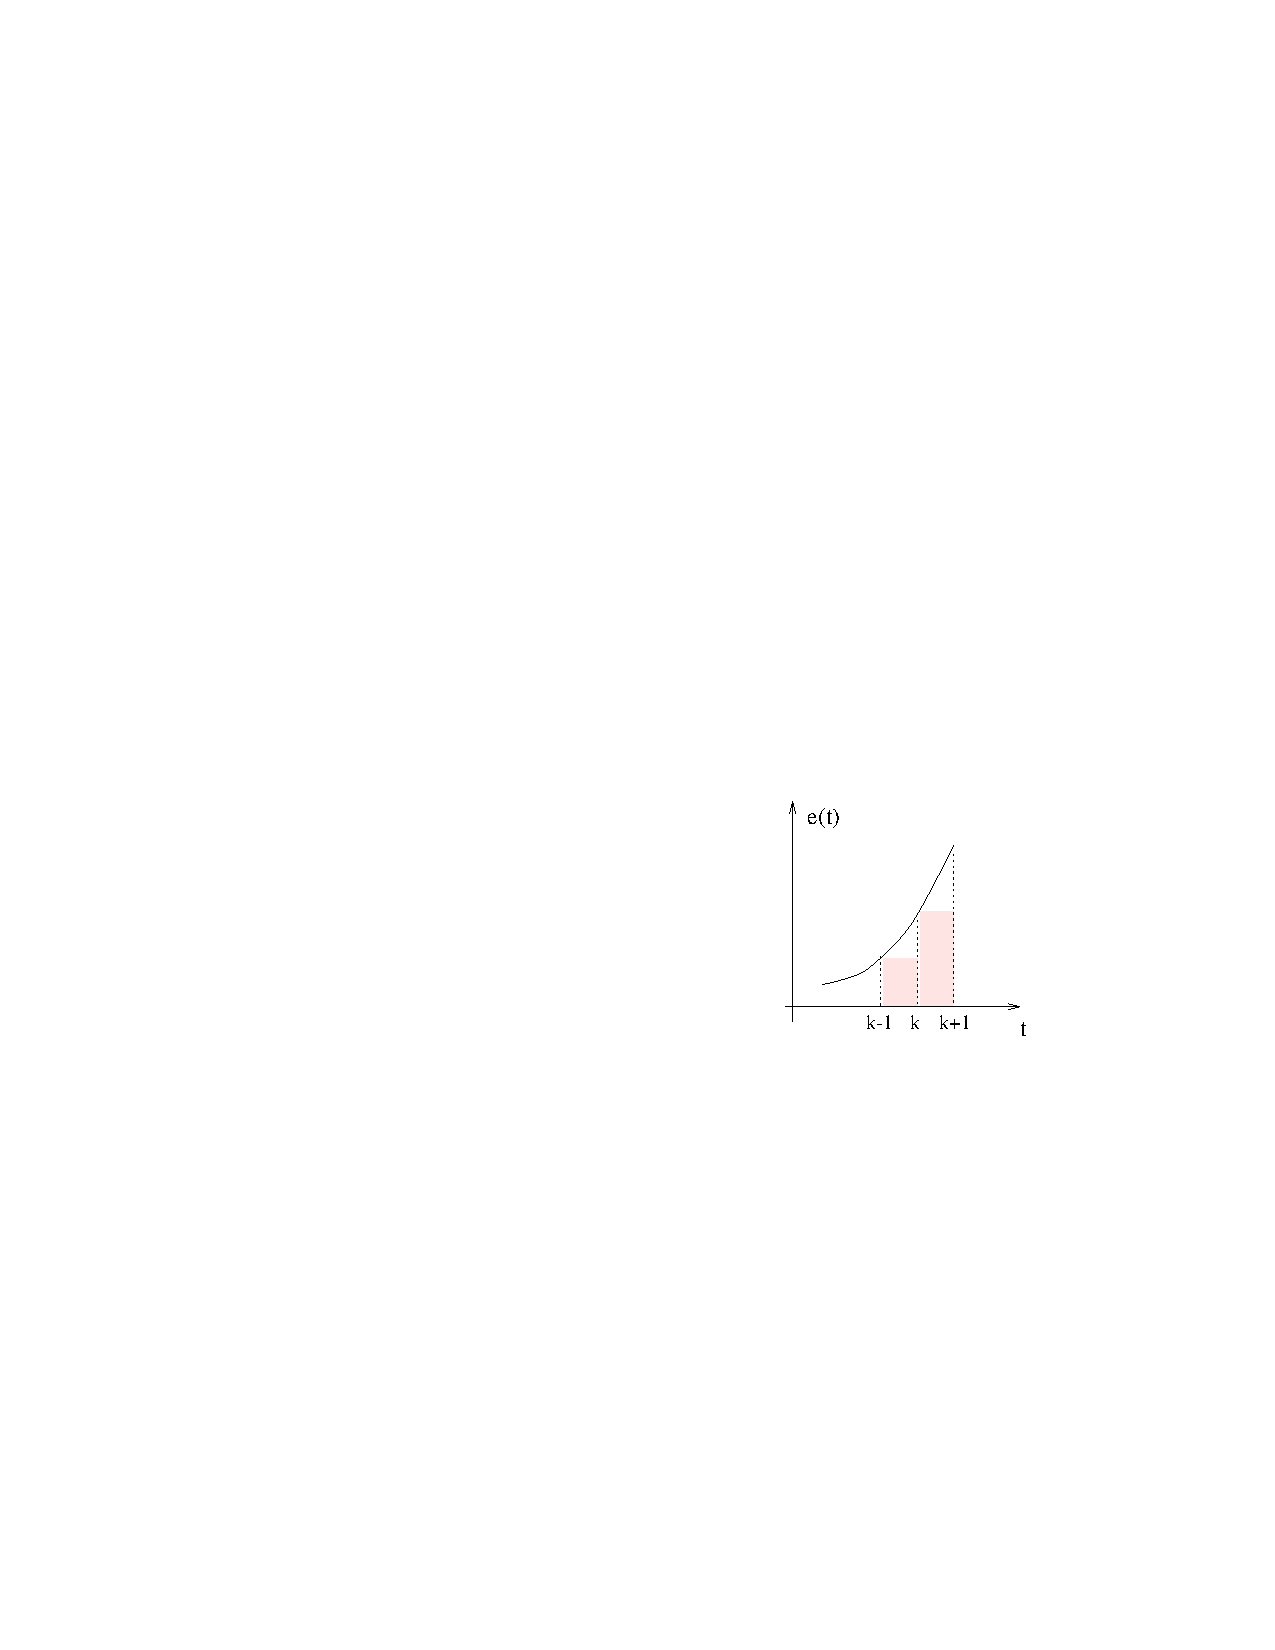
\includegraphics[width=1\linewidth]{F_euler}
			\end{figure}
		\end{column}
	\end{columns}
\end{frame}

\begin{frame}
	\frametitle{Forward rectangular rule}
	\begin{block}{Mathematical approach}
		From equation (8.1) we have that
		\begin{center}
			$u(kT_s) = u\big((k-1)T_s \big) + T_s e \big((k-1)T_s \big)$\\
		\end{center}
		By taking the $\mathcal{Z}$-transform we obtain the discrete equivalent of H(s),
		\vspace{-1em}
		\begin{center}
			$U(z) = z^{-1}U(z) + T_s z^{-1}E(z)$ \hspace{0.5em} $\Leftrightarrow$ \hspace{0.5em} \\$(1 - z^{-1})U(z) = T_s z^{-1} E(z)$ \hspace{0.5em} $\Leftrightarrow$ \hspace{0.5em} $\frac{z-1}{T_s}U(z) = E(z)$
		\end{center}
		This means that we need to apply the following substitution in order to discretize a given continuous-time transfer function:
		\begin{center}
			$s \gets \frac{z-1}{T_s}$ (8.2)
		\end{center}
	\end{block}
\end{frame}

\begin{frame}
	\frametitle{Backward rectangular rule (=Backward Euler)}
\begin{columns}
	\begin{column}{0.5\textwidth}
	\begin{block}{General approach}
		The area is approximated by the rectangle looking \textbf{backward} from $k$ toward $(k-1)$ with an amplitude equal to the value of the function at $k$. 
	\end{block}	
	\end{column}
		
	\begin{column}{0.5\textwidth}
		\begin{figure}
			\centering
			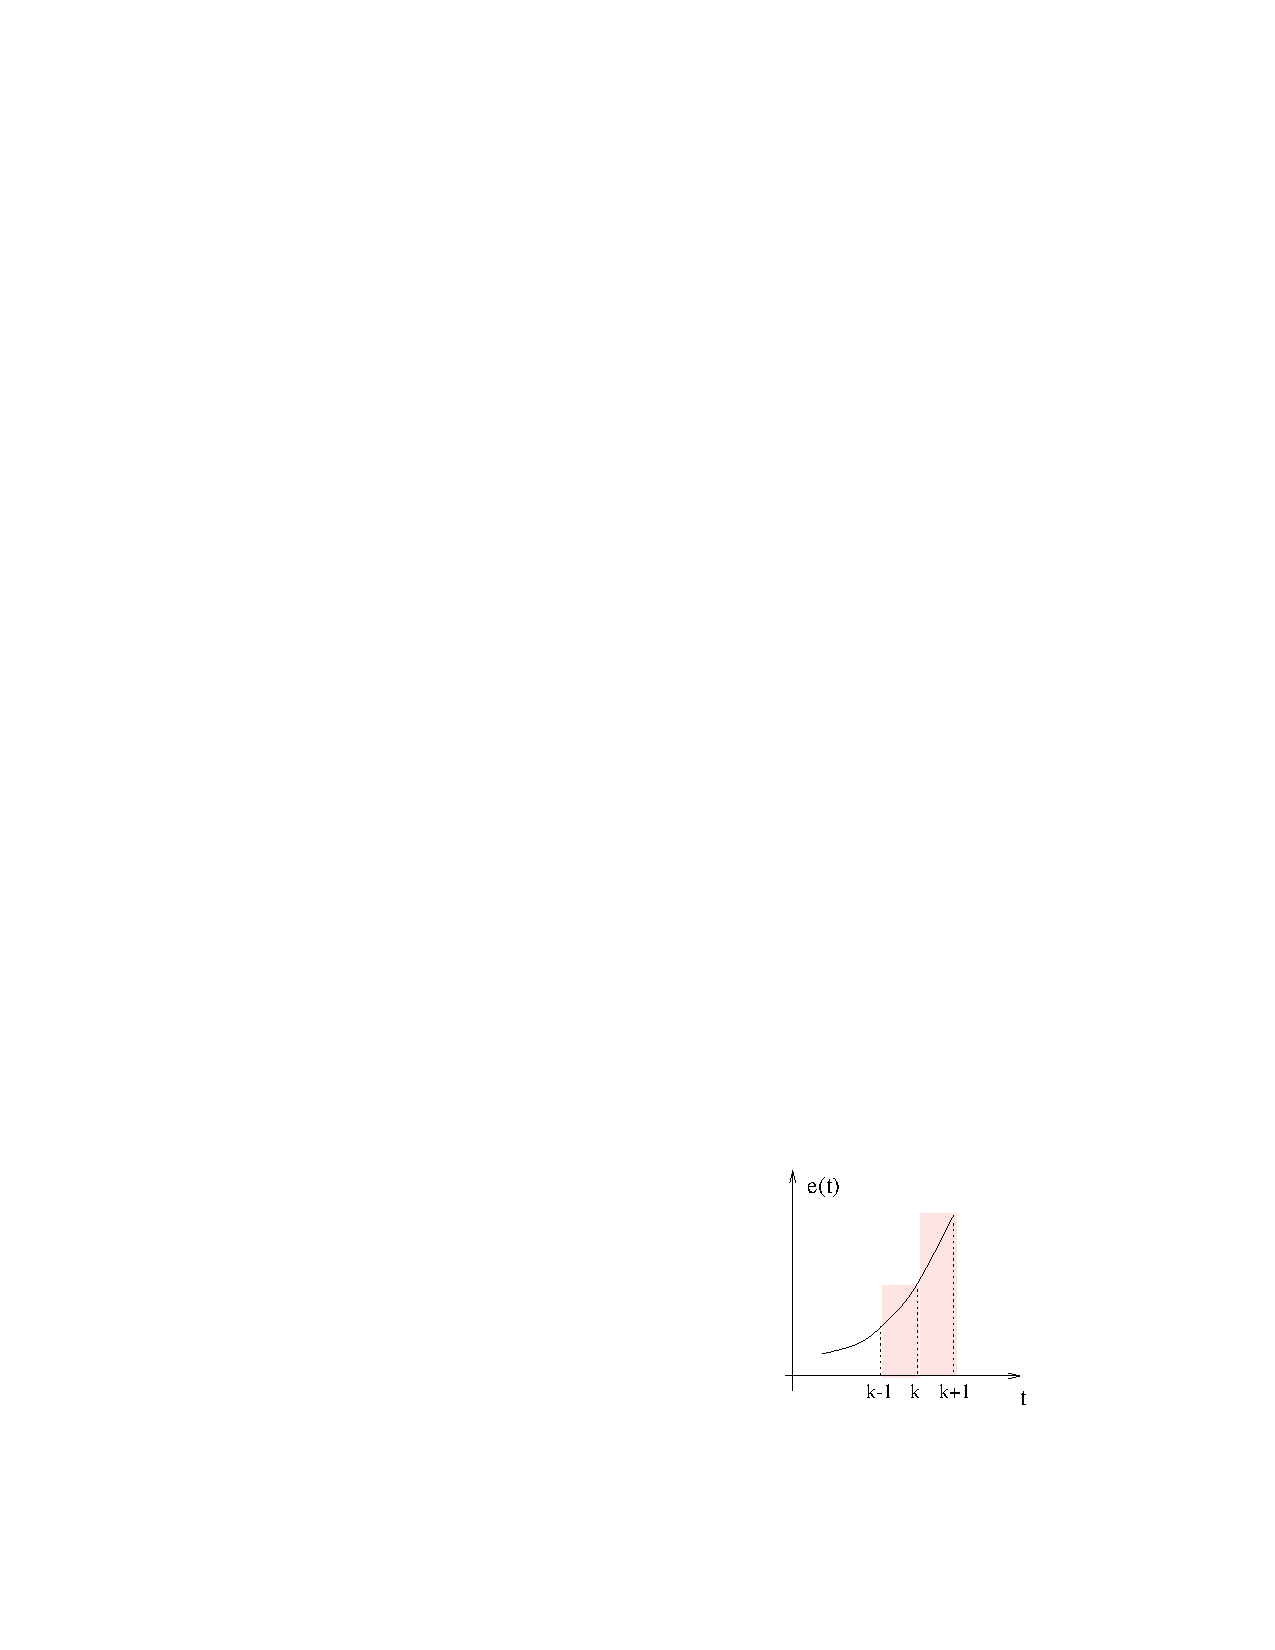
\includegraphics[width=1\linewidth]{B_euler}
		\end{figure}
	\end{column}
\end{columns}
\end{frame}

\begin{frame}
	\frametitle{Backward rectangular rule}
	\begin{block}{Mathematical approach}
		From equation (8.1) we have that
		\begin{center}
			$u(kT_s) = u\big((k-1)T_s \big) + T_s e \big(kT_s \big)$\\
		\end{center}
		By taking the $\mathcal{Z}$-transform we obtain the discrete equivalent of H(s),
		\vspace{-1em}
		\begin{center}
			$U(z) = z^{-1}U(z) + T_s E(z)$ \hspace{0.5em} $\Leftrightarrow$ \hspace{0.5em} \\$(1 - z^{-1})U(z) = T_s E(z)$ \hspace{0.5em} $\Leftrightarrow$ \hspace{0.5em} $\frac{z-1}{zT_s}U(z) = E(z)$
		\end{center}
		This means that we need to apply the following substitution in order to discretize a given continuous-time transfer function:
		\begin{center}
			$s \gets \frac{z-1}{zT_s}$ (8.3)
		\end{center}
	\end{block}
\end{frame}

\begin{frame}
	\frametitle{Bilinear rule (= trapezoidal or Tustin rule)}
\begin{columns}
	\begin{column}{0.5\textwidth}
		\begin{block}{General approach}
			This method makes use of the area of the \textbf{trapezoid} formed by the average of the selected rectangles used in the forward and backward rectangular rule.Thus the amplitude equal to the value of the function at $(k-1)$ and the amplitude equal to the value of the function at $(k)$ are connected by a line as shown in the illustration.
		\end{block}	
	\end{column}

	\begin{column}{0.5\textwidth}
		\begin{figure}
			\centering
			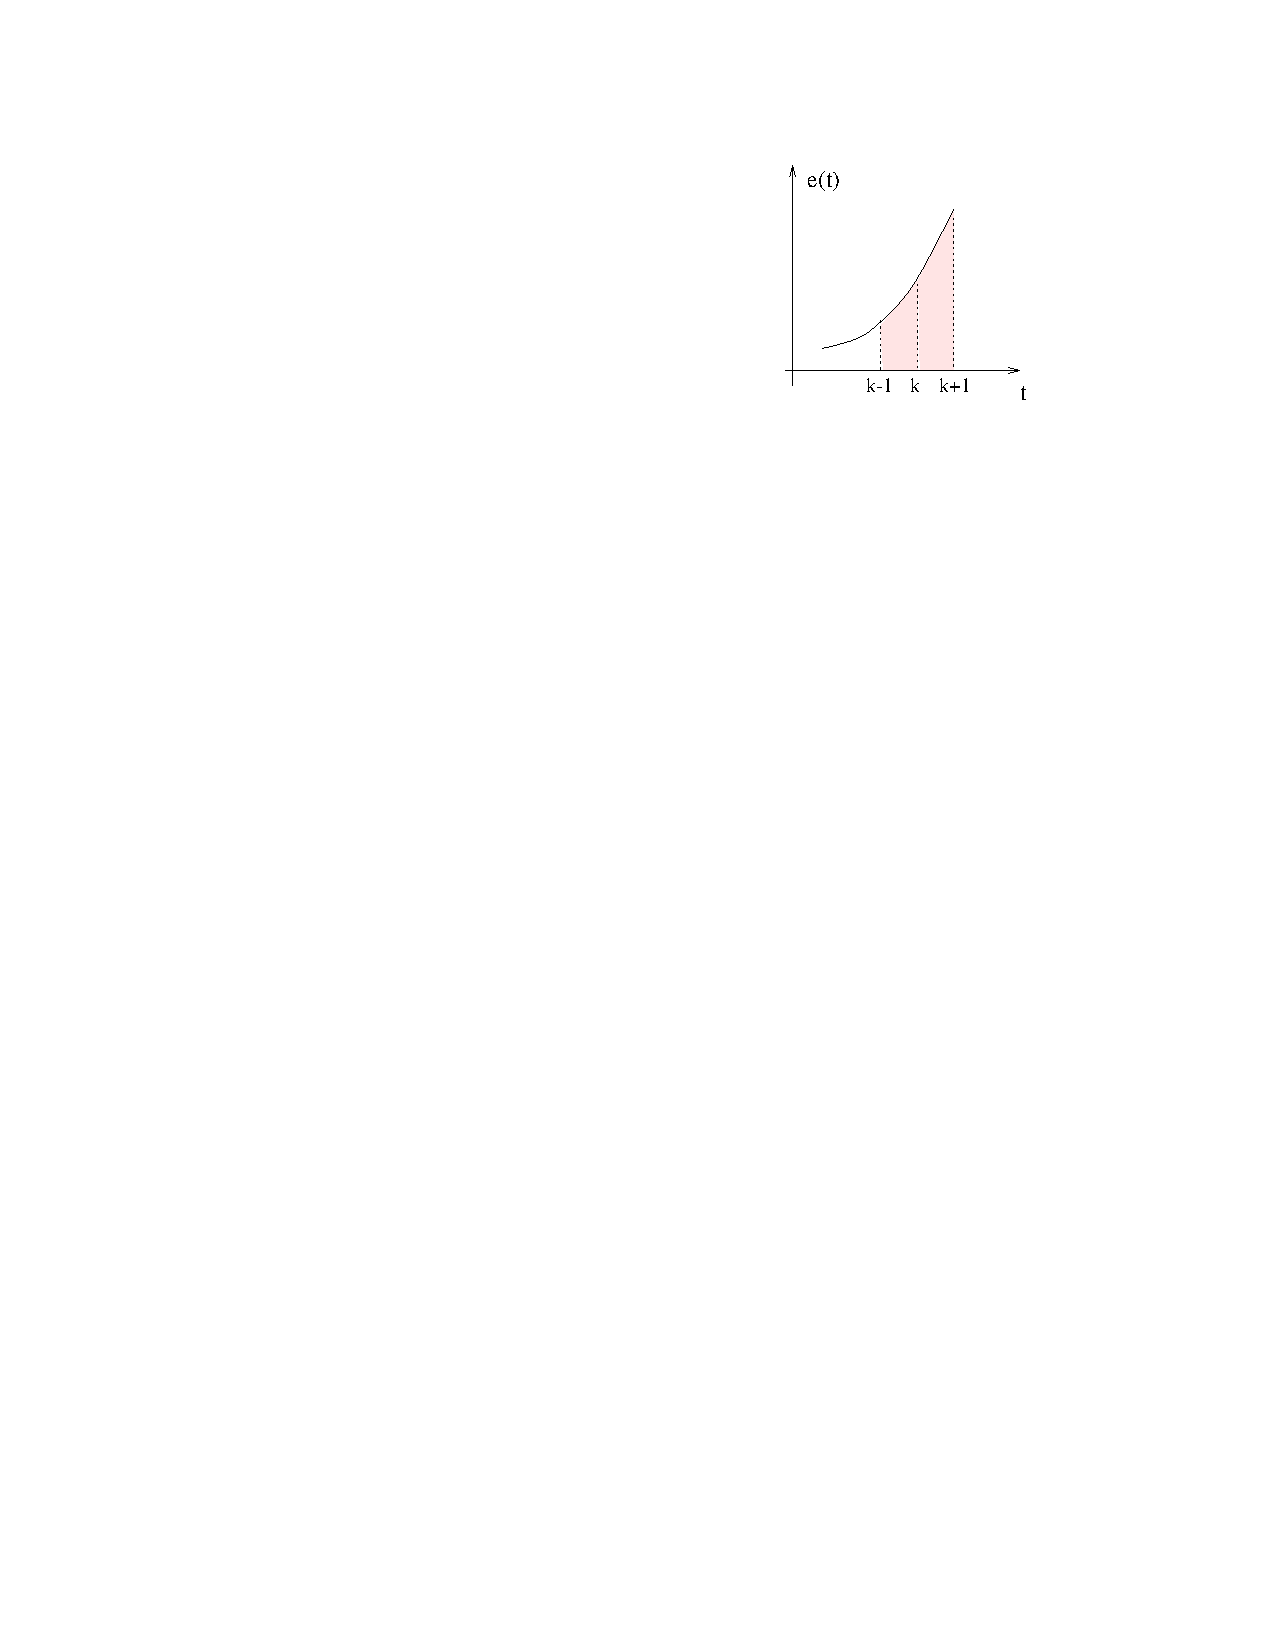
\includegraphics[width=1\linewidth]{T_euler}
		\end{figure}
	\end{column}	
\end{columns}
\end{frame}

\begin{frame}
	\frametitle{Bilinear transformation}
	\begin{block}{Mathematical approach}
		From equation (8.1) we have that
		\vspace{-1em}
		\begin{center}
			$u(kT_s) = u\big((k-1)T_s \big) + T_s \frac{e(kT_s) + e \big((k-1)T_s\big)}{2}$\\
		\end{center}
		By taking the $\mathcal{Z}$-transform we obtain the discrete equivalent of H(s),
		\vspace{-1em}
		\begin{center}
			$U(z) = z^{-1}U(z) + \frac{T_s}{2} \big( E(z) + z^{-1}E(z) \big)$ \hspace{0.5em} $\Leftrightarrow$ \hspace{0.5em} \
			\ $(1 - z^{-1})U(z) = \frac{T_s}{2} (1 + z^{-1}) E(z)$ \hspace{0.5em} $\Leftrightarrow$ \hspace{0.5em} $\frac{2}{T_s}\frac{z-1}{z+1}U(z) = E(z)$
		\end{center}
		This means that we need to apply the following substitution in order to discretize a given continuous-time transfer function:
		\begin{center}
			$s \gets \frac{2}{T_s}\frac{z-1}{z+1}$ (8.4)
		\end{center}
	\end{block}
\end{frame}

\begin{frame}
	\frametitle{Bilinear rule}
	\begin{example}
		Given:
		\begin{center}
			$H(s) = \frac{s + 1}{0.1s + 1}$
		\end{center}
		We now apply substitution (8.4):
		\begin{center}
			$H(z) = \frac{(2 + T)(T - 2)z^{-1}}{(0.2 + T) + (T - 0.2)z^{-1}}$
		\end{center}
		Using T=0.25s, this results in:
		\begin{center}
			$H(z) = \frac{5(z - 0.7778)}{z + 0.1111}$
		\end{center}
	\end{example}
\end{frame}

\begin{frame}
	\frametitle{Discretization of state-space models}
	\begin{block}{General approach applied on Forward Euler}
		Given the following continuous-time model in state-space form:
		\vspace{-2em}
		\begin{center}
			\begin{align*}
			\dot{x} &= Ax + Bu  & sX &= AX + BU\\
			y &= Cx + Du & Y &= CX + DU
			\end{align*}
		\end{center}
		If we use the Forward Euler method, we have that $s$ is replaced by $\frac{z-1}{T_s}$, so we can find the discrete-time equivalent as follows:
		\vspace{-2em}
		\begin{center}
			\begin{align*}
			\frac{z-1}{T_s} X &= AX + BU\\
			Y &= CX + DUç
			\end{align*}
		\end{center}
	\end{block}
\end{frame}

\begin{frame}
	\frametitle{Discretization of state-space models}
	\begin{block}{General approach applied on Forward Euler}
		Which leads to the following
		\vspace{-2em}
		\begin{center}
			\begin{align*}
			zX &= (I - AT_s)X + BT_sU\\
			x(k+1) &= (I - AT_s)x(k) + (BT_s)u(k)\\
			x(k+1) &= A_d x(k) + B_d u(k)
			\end{align*}
		\end{center}
		The output equation $Y = CX + DU$ remains.
	\end{block}
\end{frame}

\begin{frame}
	\frametitle{Discretization of state-space models}
	\begin{block}{State-space models}
		A similar calculation can be done for the backward rectangular rule and the bilinear transformation resulting in the following table:
		\begin{center}
			\begin{figure}
				\centering
				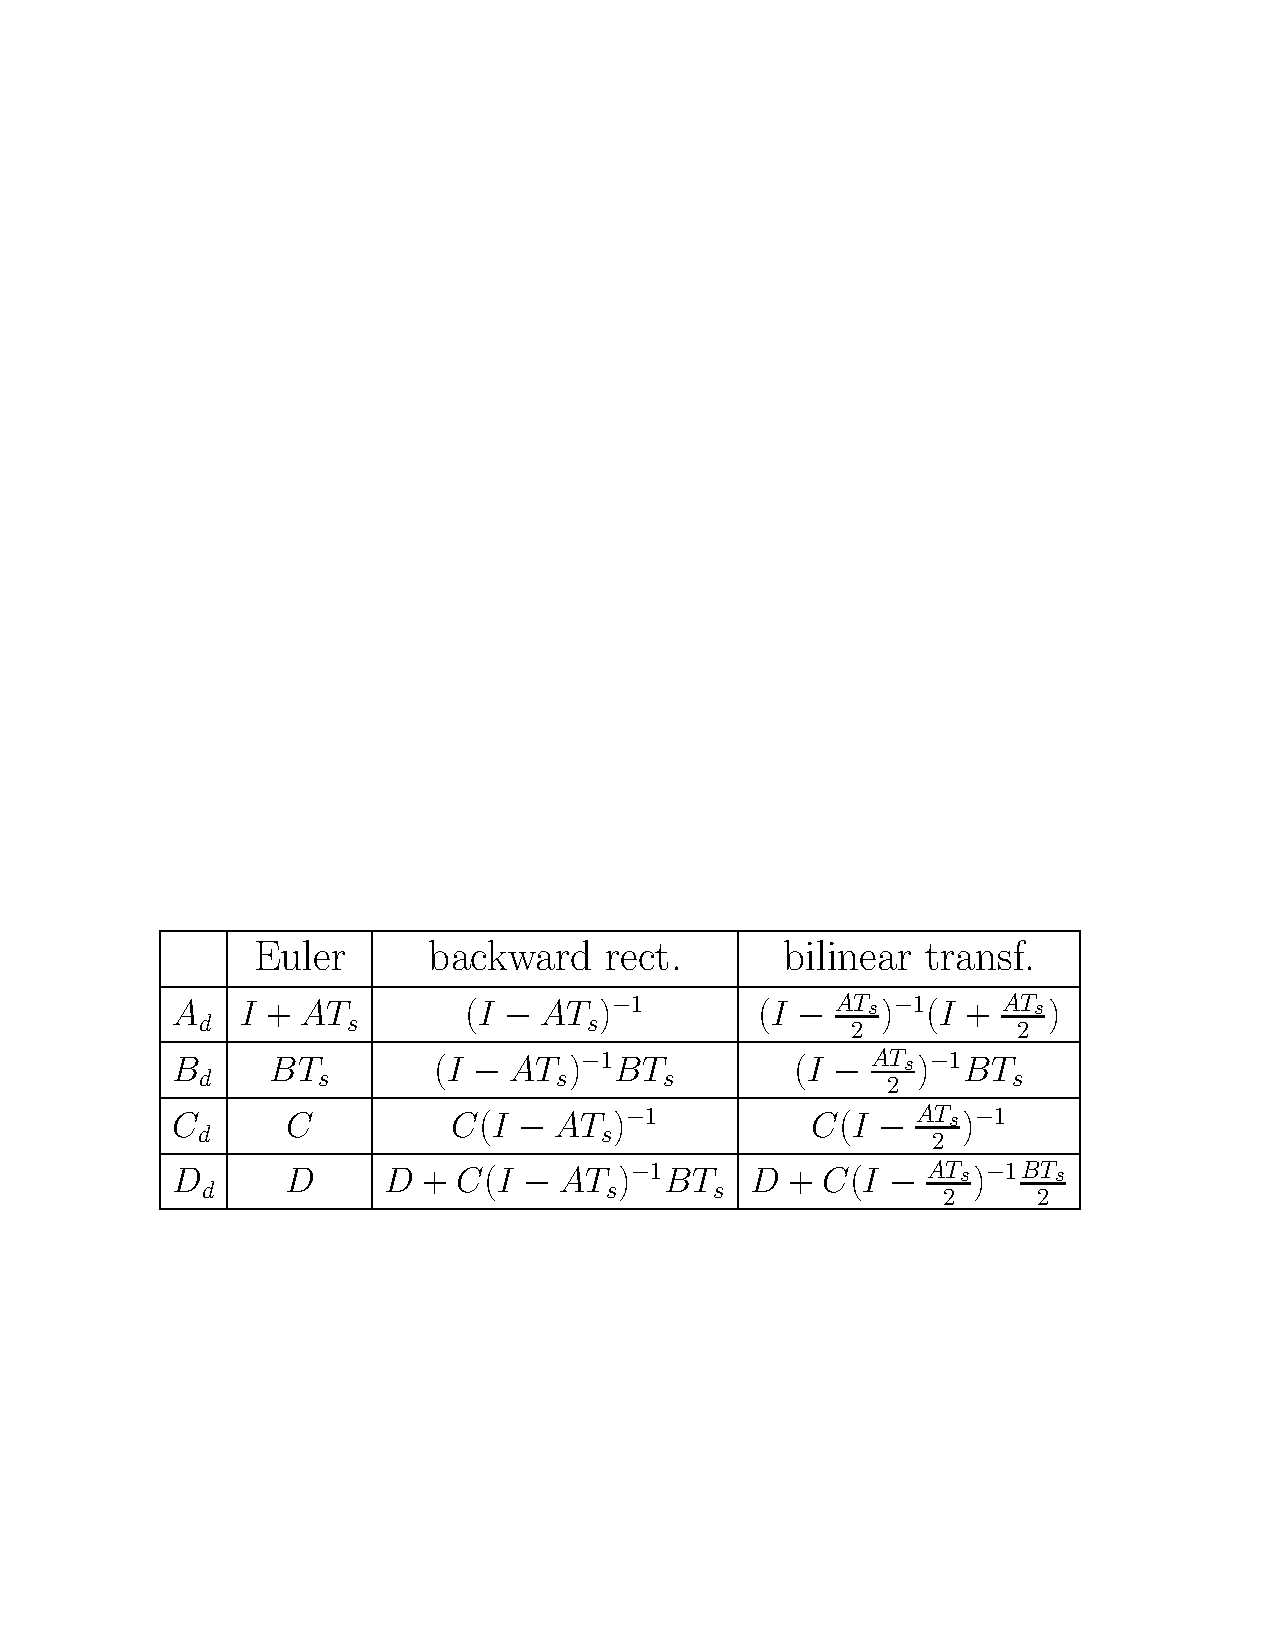
\includegraphics[width=1\linewidth]{Steady_State}
			\end{figure}
		\end{center}
	\end{block}
\end{frame}

\begin{frame}
	\frametitle{Stability of the numerical integration methods}
	\begin{block}{Stability}
		As already mentioned, a discrete system is stable when its poles lie within the unit circle of the z-plane and a continuous system is stable when its poles have a negative real part in the s-plane. Subsequently the $(s=j\omega)$-axis is the boundary between poles of stable and unstable continuous systems.\\
		\vspace{1em}
		Each of the discretization methods can be considered as a map from the s-plane to the z-plane. It is interesting to know how the $j\omega$-axis is mapped by every rule and where the stable part of the s-plane appears in the z-plane. This can be realized by solving formulas (8.2-8.3) to z and replacing s by $j\omega$. 
	\end{block}
\end{frame}

\begin{frame}
	\frametitle{Stability of the numerical integration methods}
	\begin{block}{Boudaries of the stable regions}
		Expressions of z in terms of s:
		\begin{itemize}
			\item $z = 1 + T_ss$
			\item $z = \frac{1}{1 - T_ss}$
			\item $z = \frac{1 + T_s\frac{s}{2}}{1 - T_s\frac{s}{2}}$
		\end{itemize}
		By substituting s by $j\omega$ the boundaries of the regions in the z-plane, which originate from the stable portion of the s-plane, are obtained.
	\end{block}
\end{frame}

\begin{frame}
	\frametitle{Stability of the numerical integration methods}
	\begin{block}{Graphical representation}
		Stable s-plane poles map onto the shaded regions in the z-plane. The unit circle is shown for reference.
	\begin{figure}
		\centering
		\includegraphics[width=0.85\linewidth]{Stabiliteit}
	\end{figure}
	\end{block}
\end{frame}

\begin{frame}
	\frametitle{Stability of the numerical integration methods}
	\begin{block}{Mapping of the left-hand-s-plane}
		\begin{itemize}
			\item Forward Euler: a stable continuous-time system may become unstable after discretization;\\
			\item Backward Euler: a stable continuous-time system will stay stable after discretization, but the number of degrees of freedom is restricted;\\
			\item Bilinear transformation: the entire left-hand-plane is mapped into the unit circle.\\
		\end{itemize}
	\end{block}
\end{frame}

\begin{frame}
	\frametitle{Bilinear rule with prewarping}
	\begin{alertblock}{Distortion}
		Looking at the graphical representation of the stability on the previous slide, you can see that the bilinear rule maps the stable region of the s-plane into the stable region of the z-plane. The entire $j\omega$-axis is compressed into the $2\pi$-length of the unit circle, causing a frequency distortion.
	\end{alertblock}
	\begin{block}{Origin of prewarping}
		On the next slide you can see that when we compare the $\mathcal{Z}$-transform with the bilinear transformation, points $b$ and $d$ in the s-plane are mapped onto different points in the z-plane. $(-1 + 0j)$ can only be reached by the bilinear rule when $\omega$ goes to infinity.
	\end{block}
\end{frame}

\begin{frame}
	\frametitle{Bilinear rule with prewarping}
	\begin{block}{Origin of prewarping}
		\begin{figure}
			\centering
			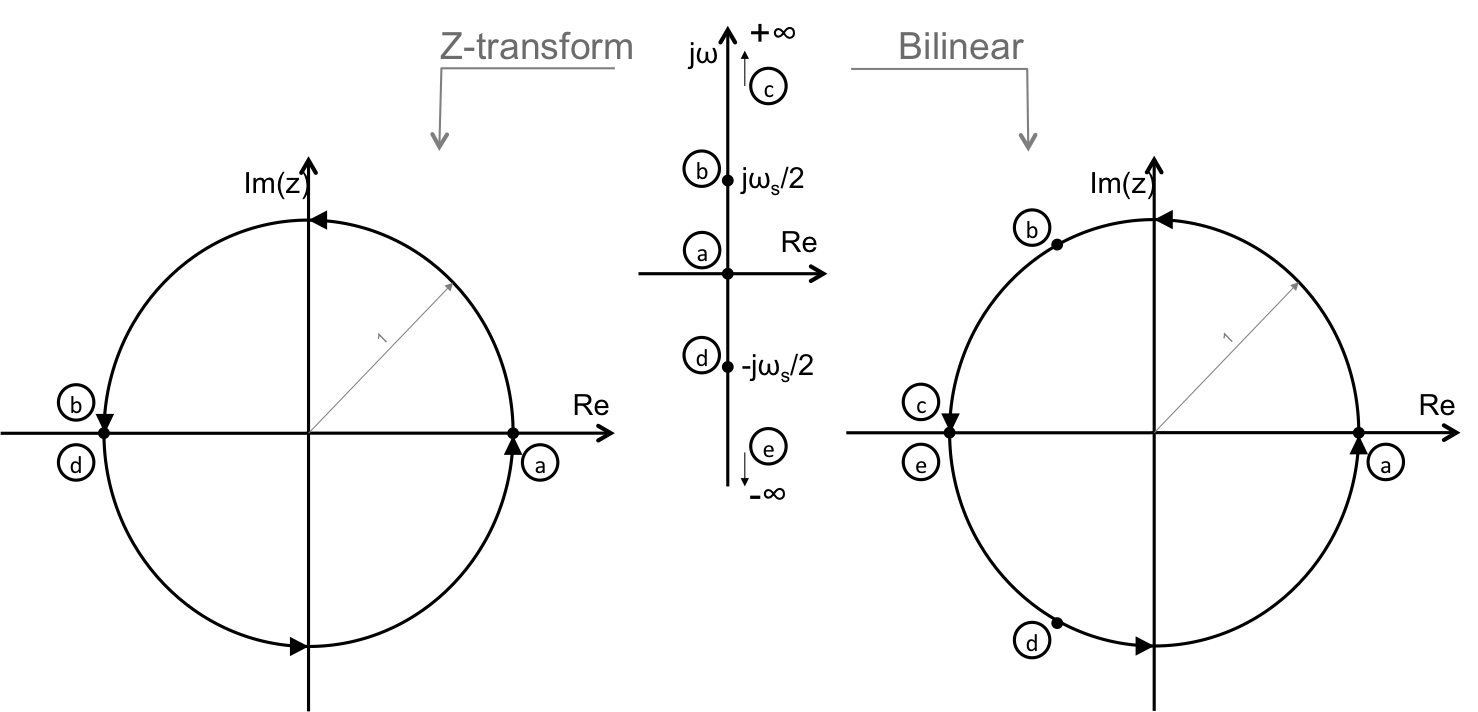
\includegraphics[width=1\linewidth]{Prewarp}
		\end{figure}
	\end{block}
\end{frame}

\begin{frame}
	\frametitle{Bilinear rule with prewarping}
	\begin{block}{Distortion: frequency domain}
		The bilinear rule causes every feature that is visible in the frequency response of the continuous-time filter to also be visible in the discrete-time filter, but at a different frequency. However, at low frequencies, the same behaviour of the function is guaranteed. This is illustrated by the figure on the next slide.\\
		\vspace{1em}
		When the actual frequency of $\omega$ is input to the discrete-time filter designed by use of the bilinear transform, it is desired to know at what frequency,  $\omega_a$, for the continuous-time filter that this  $\omega$ is mapped to.
	\end{block}
\end{frame}

\begin{frame}
	\frametitle{Bilinear rule with prewarping}
	\vspace{-0.5em}
	\begin{figure}
		\centering
		\includegraphics[width=0.85\linewidth]{Distortion_bode}
	\end{figure}
\end{frame}

\begin{frame}
	\frametitle{Bilinear rule with prewarping}
	\begin{block}{$\omega_a$ with input $\omega$}
		We now look for a relation between $\omega_a$ and $\omega$, using the 's-domain'-\\'z-domain' relation $z = e^{sT}$ and the substitution $s=j\omega$:
		\vspace{-2em} 
		\begin{center}
			\begin{align*}
			\big(\frac{2}{T} \frac{z-1}{z+1}\big)_{z = e^{j\omega T}} &=\frac{2}{T} \frac{e^{j\omega T}-1}{e^{j\omega T}+1}\\
			&= \frac{2}{T} \frac{e^{j\omega T/2} (e^{j\omega T/2} - e^{-j\omega T/2})}{e^{j\omega T/2}(e^{j\omega T/2} + e^{-j\omega T/2})}\\
			&= j \frac{2}{T} \frac{sin(\omega T/2)}{cos(\omega T/2)}\\
			&= j \frac{2}{T} tan(\frac{\omega T}{2}) = j\omega_a
			\end{align*}
		\end{center}
	\end{block}
\end{frame}

\begin{frame}
	\frametitle{Bilinear rule with prewarping}
	\begin{block}{Frequency warping}
		The discrete-time system has the same behavior at frequency $\omega$ as the continuous-time system at frequency $\omega_a = \frac{2}{T} tan(\frac{\omega T}{2})$. \\ 
		\vspace{1em}
		Specifically, the gain and phase shift that the discrete-time filter has at frequency $\omega$ is the same gain and phase shift that the continuous-time filter has at frequency  $\omega_a = \frac{2}{T} tan(\frac{\omega T}{2})$.\\
		\vspace{1em}
		This effect of the non-linear relation between $\omega$ and $\omega_a$ is called \textbf{frequency warping}.
	\end{block}
\end{frame}

\begin{frame}
	\frametitle{Bilinear rule with prewarping}
	\begin{block}{Frequency prewarping}
		In certain situations, however, we really want the characteristics to be conserved during the discretization.\\
		\vspace{1em}
		By setting $\omega_a = \frac{2}{T} tan(\frac{\omega T}{2})$ for every frequency specification that the designer has control over, the frequency warping will be compensated. This is called \textbf{frequency prewarping}.\\
		\vspace{1em}
		The digital filter can be made to match the frequency response of the continuous filter at frequency  $\omega_0$  if the following transformation is substituted into the continuous filter transfer function:
		\begin{center}
			$s \gets \frac{\omega_0}{tan\big(\frac{\omega_0T_s}{2}\big)} \frac{z-1}{z+1}$ (8.4)
		\end{center}
	\end{block}
\end{frame}

\begin{frame}
	\frametitle{Bilinear rule with prewarping}
	\vspace{-0.5em}
	\begin{figure}
		\centering
		\includegraphics[width=0.8\linewidth]{Distortion_bode1}
	\end{figure}
\end{frame}

\subsection{Impulse Invariant Method}

\begin{frame}
	\frametitle{Impulse-invariant method}
	\begin{block}{Practical rule}
		This method converts a continuou-time s system into a discrete one by matching the impulse response using these transformations:
		\vspace{-1em}
		\begin{center} 
			\begin{tabular}{ | l | c |} 
			\hline $H(s)$ & $H(z)$, $a = e^{bT_s}$\\ 
			\hline $\frac{c}{s - b}$ & $\frac{T_sc}{1 - az^{-1}}$\\ 
			\hline $\frac{c}{(s - b)^2}$ & $T_s^2 \frac{caz^{-1}}{(1 - az^{-1})^2}$ \\
			\hline $\frac{c}{(s - b)^3}$ & $\frac{T_s^3 caz^{-1}(1 + az^{-1})}{2(1 - az^{-1})^3}$ \\
			\hline $\frac{c}{(s - b)^4}$ & $\frac{T_s^4 caz^{-1}(1 + 4az^{-1} + a^2z^{-2})}{6(1 - az^{-1})^4}$ \\
			\hline 
			\end{tabular}
		\end{center}
	\end{block}
\end{frame}

\subsection{Zero-pole Equivalent}

\begin{frame}
	\frametitle{Zero-pole equivalent}
	\begin{block}{General approach}
		The map $z = e^{sT}$ is applied to the poles as well as to the zeros of the continuous system. The following rules must be followed:
		\begin{enumerate}
			\item If $s=-a$ is a pole of H(s), then $z=e^{-aT}$;
			\item All finite zeros $s=-b$ are mapped by $z = e^{-bT}$;
			\item Zeros at $\infty$ are mapped to $z = -1$;
			\item The DC gain is set such that $\lim_{s \to 0} G(s) = \lim_{z \to 1} G_d(z)$.
		\end{enumerate}
	\end{block}
\end{frame}

\begin{frame}
	\frametitle{Zero-pole equivalent}
	\begin{example}
		Given:
		\begin{center}
			$H(s) = \frac{s + 1}{0.1s + 1}$
		\end{center}
		Pole at $s=-10$ and zero at $s=-1$.
		
		New discrete transfer function with equivalent poles and zeros:
		\begin{center}
			$H(z) = K \frac{z - e^{-T}}{z - e^{-10T}}$
		\end{center}
		K is chosen so that $\mid H(z)\mid _{z=1} = \mid H(s) \mid _{s=0} \to K=4.150$

		Using $T=0.25$, this results in:
		\begin{center}
			$H(z) = 4.150 \frac{z-0.7788}{z-0.0821}$
		\end{center}
	\end{example}
\end{frame}


\subsection{Hold Equivalent}
\begin{frame}
	\frametitle{Hold equivalent}
	\begin{block}{General approach}
		This method uses a discrete system consisting of 3 subsystems, each with its own purpose. 
		\begin{enumerate}
			\item Hold: approximating $e(t)$ from the samples $e[k]$
			\item H(s): putting the $e(t)$ through the given transfer function H(s) of the continuous system, resulting in u(t)
			\item Sampler: sampling u(t) 
		\end{enumerate}
		\vspace{-1em}
		\begin{figure}
			\centering
			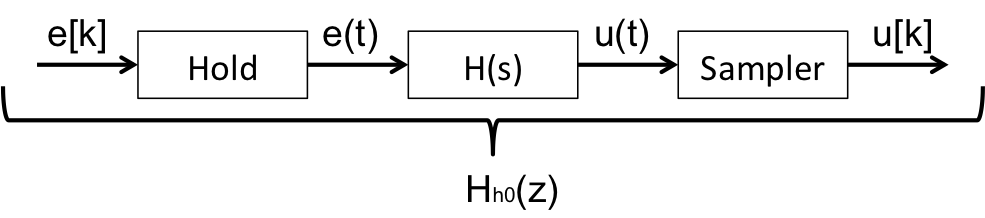
\includegraphics[width=0.8\linewidth]{hold_equivalent}
		\end{figure}
		\vspace{-1em}
		There are many techniques for holding a sequence of samples.
	\end{block}
\end{frame}

\begin{frame}
	\frametitle{Zero-order hold equivalent (ZOH)}
\begin{columns}
	\begin{column}{0.5\textwidth}
	\begin{block}{Practical rule}
		The zero-order hold equivalent transfer function $H_{zoh}(z)$ can be found by computing the following:
		\begin{center}
			$H_{zoh}(z) = (1 - z^{-1}) \mathcal{Z}\{\frac{H(s)}{s}\}$
		\end{center}
		This is obtained by holding e(t) constant at e(k) over the interval $kT_s$ to $(k+1)T_s$ and $\mathcal{Z}$-transforming it.
	\end{block}
	\end{column}
	
	\begin{column}{0.5\textwidth}
		\begin{figure}
			\centering
			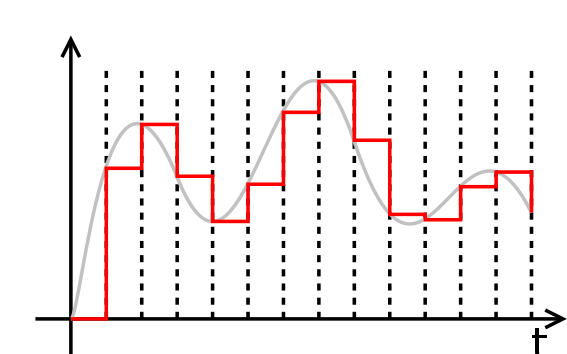
\includegraphics[width=1\linewidth]{zero-order}
		\end{figure}
	\end{column}
\end{columns}
\end{frame}

\begin{frame}
	\frametitle{Zero-order hold equivalent}
	\begin{example}
		\begin{center}
			$H(s) = \frac{0.1}{s + 0.1}$
		\end{center}
		Step 1: multiply by 1/s and perform partial fraction expansion
		\begin{center}
			$\frac{H(s)}{s} = \frac{0.1}{s * (s + 0.1)} = \frac{1}{s} - \frac{1}{s + 0.1}$
		\end{center}
		Step 2: perform z-transformation
		\begin{center}
			$\mathcal{Z} \{\frac{H(s)}{s}\} = \frac{1}{1 - z^{-1}} - \frac{1}{1 - e^{-0.1T} * z^{-1}}$
		\end{center}
		Step3: simplify and multiply by $(1-z^{1})$
		\begin{center}
			$H_{ho}(z) = \frac{1 - e^{-0.1T}}{z - e^{0.1T}}$
		\end{center}
	\end{example}
\end{frame}

\begin{frame}
	\frametitle{Zero-order hold equivalent}
	\begin{block}{Step Invariant Transformation}
		This rule is also called the step-invariant method because it matches the step response of the continuous and the discrete system. Next transformations may be useful:
		\vspace{-1em}
		\begin{figure}
			\centering
			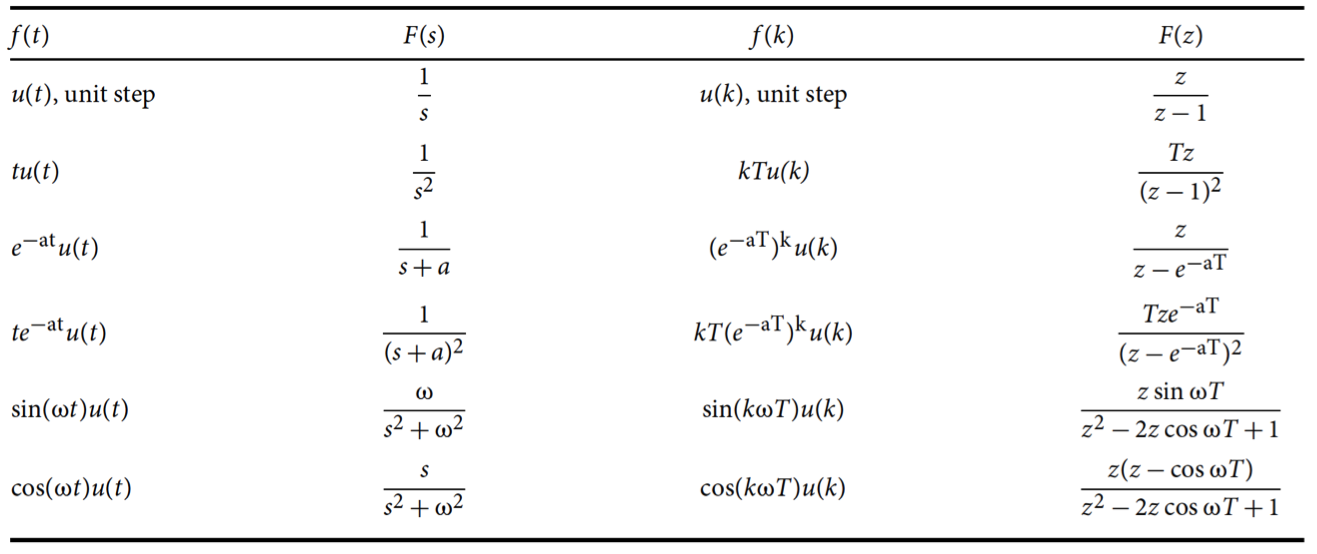
\includegraphics[width=0.85\linewidth]{step_inv}
		\end{figure}
	\end{block}
\end{frame}

\begin{frame}
	\frametitle{First-order hold equivalent}
\begin{columns}
	\begin{column}{0.5\textwidth}
	\begin{block}{Practical rule}
		The non-causal first-order hold equivalent transfer function $H_{tri}(z)$ can be found by computing the following:
		\begin{center}
			$H_{tri}(z) = \frac{(z-1)^{2}}{Tz} \mathcal{Z}\{\frac{H(s)}{s^{2}}\}$
		\end{center}
	\end{block}
	\end{column}
	
	\begin{column}{0.5\textwidth}
		\begin{figure}
			\centering
			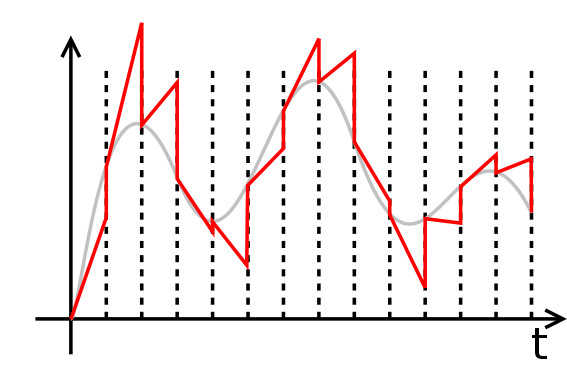
\includegraphics[width=1\linewidth]{first-order}
		\end{figure}
	\end{column}
\end{columns}
\end{frame}

\begin{frame}
	\frametitle{First-order hold equivalent}
	\begin{example}
		\begin{center}
			$H(s) = \frac{1}{s^{2}}$
		\end{center}
		Step 1: multiply by $1/s^{2}$ and perform partial fraction expansion
		\begin{center}
			$H(s) = \frac{1}{s^{4}}$
		\end{center}
		Step 2: perform z-transformation
		\begin{center}
			$\mathcal{Z}\{\frac{H(s)}{s^{2}}\} = \frac{T^{3}}{6} \frac{(z^{2} + 4z +1) z}{(z-1)^{4}}$
		\end{center}
		Step 3: simplify and multiply by $\frac{(z-1)^{2}}{T*z}$
		\begin{center}
			$H_{tri}(z) = \frac{T^{2}}{6} \frac{z^{2} + 4z + 1}{(z-1)^{2}}$
		\end{center}
	\end{example}
\end{frame}

\section{Sampling Time}

\begin{frame}
	\frametitle{Sampling time $T_s$ based on the time response}
\begin{columns}
	\begin{column}{0.5\textwidth}
	\begin{block}{Rise time}
		Time needed to reach the steady state for the first time.
	\end{block}
	\begin{block}{Practical rule}
		A good rule of thumb is $T_s = \frac{T_{rise}}{10}$.
	\end{block}
	\end{column}
	
	\begin{column}{0.5\textwidth}
		\begin{figure}
			\centering
			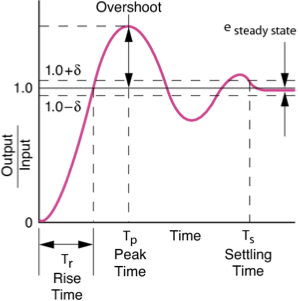
\includegraphics[width=1\linewidth]{rise_time}
		\end{figure}
	\end{column}
\end{columns}
\end{frame}

\begin{frame}
	\frametitle{Sampling time $T_s$ based on the frequency response}
	\begin{block}{Practical rule}
		A good rule of thumb is $T_s = \frac{1}{2,2Bandwidth}$.
	\end{block}
	\begin{alertblock}{Signal vs System}
		It is very important to understand that although the previous rule of thumb for a system seems the same as the rule of thumb for a signal, they differ! The rule of thumb for a signal uses the bandwidth of the signal and the rule of thumb for a system uses the bandwidth of the system, which can be found in the bodeplot or using MATLAB.
	\end{alertblock}
\end{frame}

\section{Discretization and MATLAB}
\subsection{Commands}
\begin{frame}
	\frametitle{MATLAB}
	\begin{block}{MATLAB Commands for calculations}
		MATLABs Control System Toolbox offers extensive support for discretization and re-sampling of linear systems:
	\begin{itemize}
		\item "c2d(system,sampling time,method)" used for discretization
		\item "d2c(system,sampling time,method)" used for transforming a discrete-time system to a continuous-time system (not used in the examples).
	\end{itemize}
	\vspace{1em}
		These commands can also have extra options. It is necessary to specify the options in an additional command:
		"c2dOptions('OptionName',OptionValue)".
	\end{block}
\end{frame}

\begin{frame}
	\frametitle{MATLAB}
	\begin{block}{Available options}
		\begin{itemize}
			\item 'Method'
			\item 'PrewarpFrequency'
			\item 'FractDelayApproxOrder'
		\end{itemize}
	\end{block}
	\begin{block}{Available methods}
		\begin{itemize}
			\item zero-order hold equivalent: "zoh"
			\item first-order hold equivalent: "foh"
			\item impulse invariant rule: "impuls"
			\item zero-pole matching equivalent: "matched"
			\item bilinear: "tustin"
		\end{itemize}
	\end{block}
\end{frame}

\begin{frame}
	\frametitle{MATLAB}
	\begin{block}{MATLAB Commands for visualisation}
		\begin{itemize}
			\item MATLAB can draw the bode plots of the continuous system\\ 
			$\rightarrow$ command: "bode(system)";
			\item MATLAB can carry out a graphic showing the impulse response of the continuous system and the discretized system\\
			$\rightarrow$ command: "impulse(H,'b',Hd,'r')" in which 'b' and 'r' stand for blue and red. By using colours, the step responses of both systems can easily be distinguished;
			\item MATLAB can carry out a graphic showing the step response of the continuous system and the discretized system\\
			$\rightarrow$ command: "step(H,'b',Hd,'r')".
		\end{itemize}
	\end{block}
\end{frame}

\subsection{Exercises}
\begin{frame}
	\frametitle{Exercise 1 with MATLAB}
	\begin{block}{Exercise 1}
		We will now discuss 4 methods applied on the same continuous system:
		$H(s) = \frac{s + 1}{s^{2} + s + 1}$\\
		\begin{itemize}
		\item The sampling time can be determined by the rule of thumb previously explained: $T_s$ = 2.2Bandwidth;
		\item MATLAB can calculate the bandwidth of a given continuous system, using the command: "bandwidth(system)".
		\end{itemize}
		This results in a sampling time of 0.25033 seconds for the given system
	\end{block}
\end{frame}

\begin{frame}
	\frametitle{Zero-order hold equivalent}
	\begin{example}
		Given:\\
		$H(s) = \frac{s + 1}{s^{2} + s + 1}$\\
		Sampling time = 0.25033sec\\
		\vspace{0.8em}
		MATLAB commands:
		
		H = tf([1 1],[1 1 1])	\textcolor{gray}{we define the system H by its transfer function}\\
		Hd = c2d(H,$0.25033$,'zoh') \textcolor{gray}{we calculate the discrete-time model}\\
		\vspace{0.8em}
		Result:
		$H_{zoh}(z) = \frac{0.2479z - 0.1927}{z^{2} -1.723z + 0.7785}$
	\end{example}
\end{frame}

\begin{frame}
	\frametitle{Zero-order hold equivalent (impulse and step response)}
	\vspace{-0.7em}
	\begin{columns}
		\begin{column}{0.5\textwidth}
		\begin{figure}
			\centering
			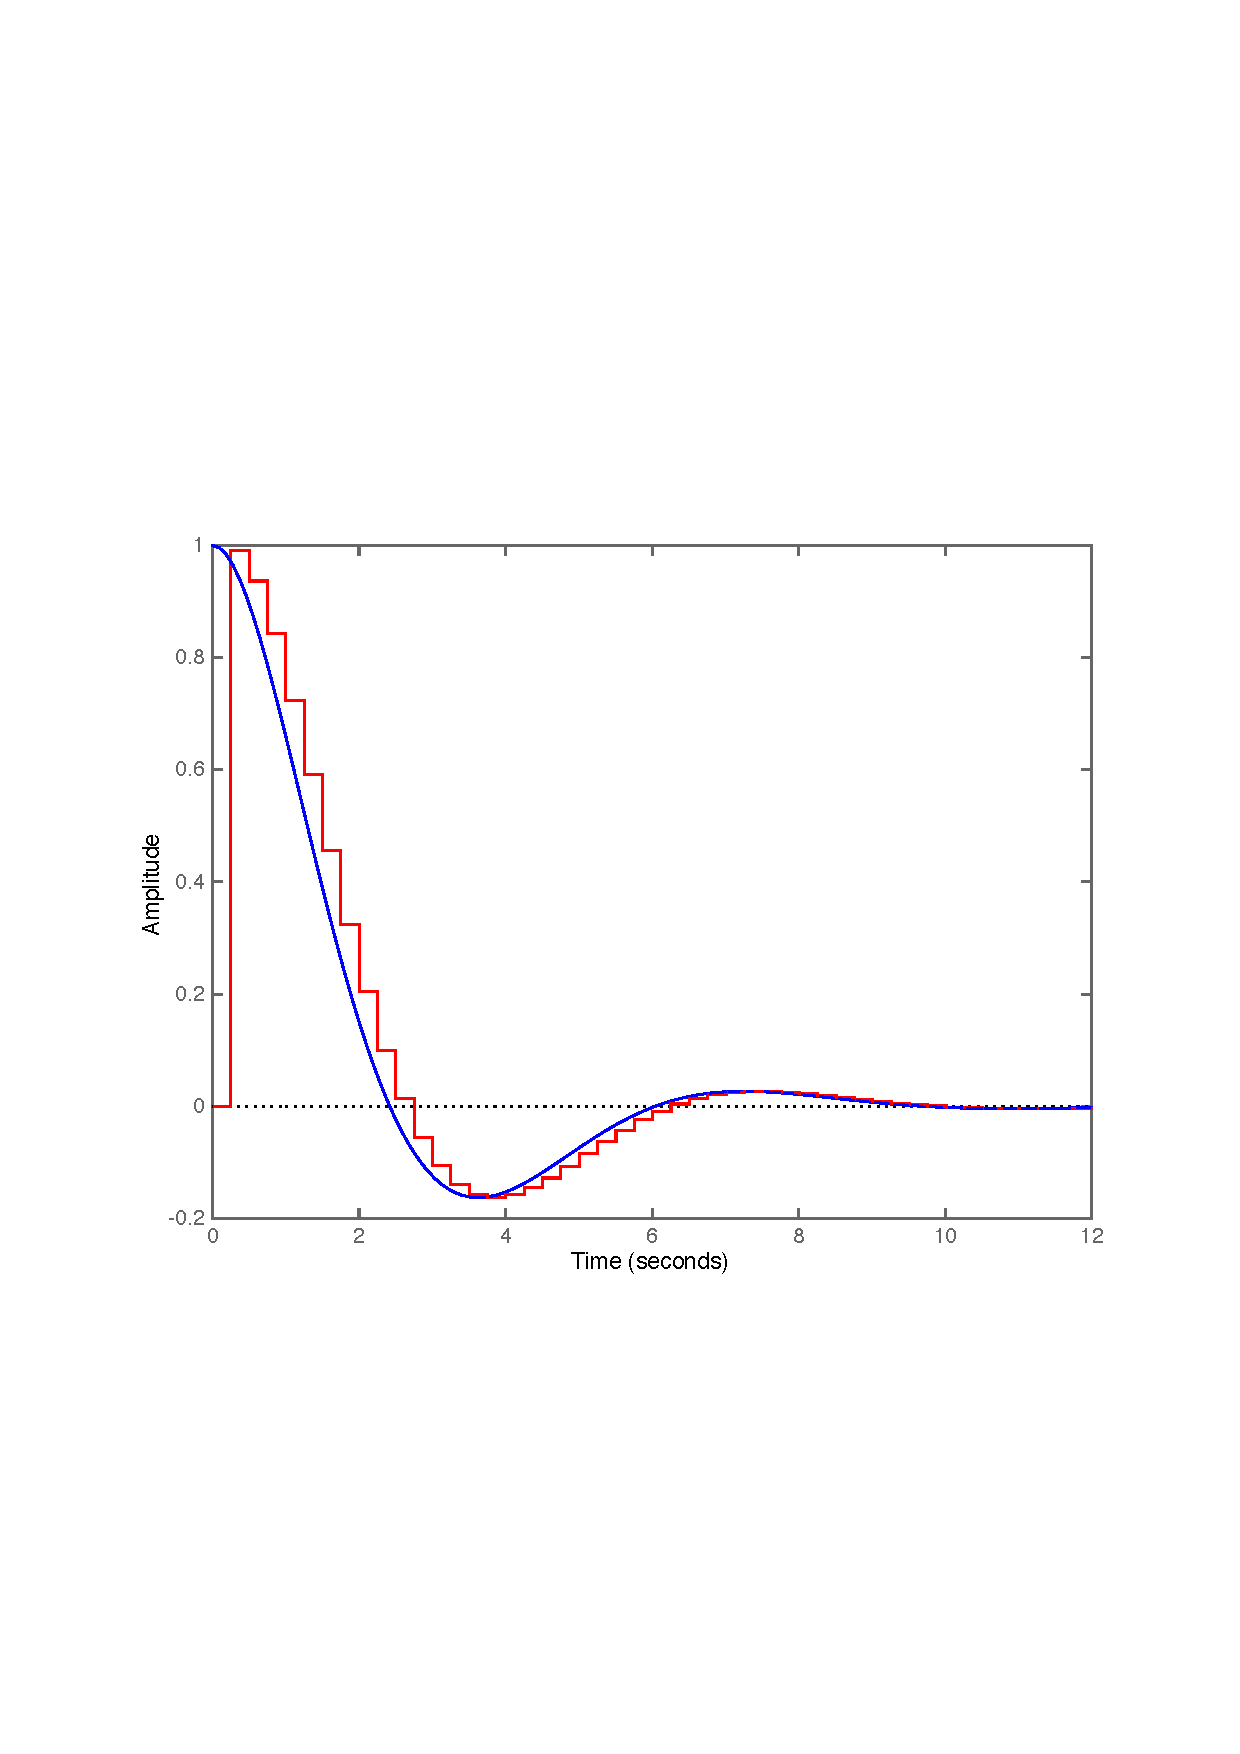
\includegraphics[width=1\linewidth]{vb1I}
		\end{figure}
		\end{column}
		\begin{column}{0.5\textwidth}
		\begin{figure}
			\centering
			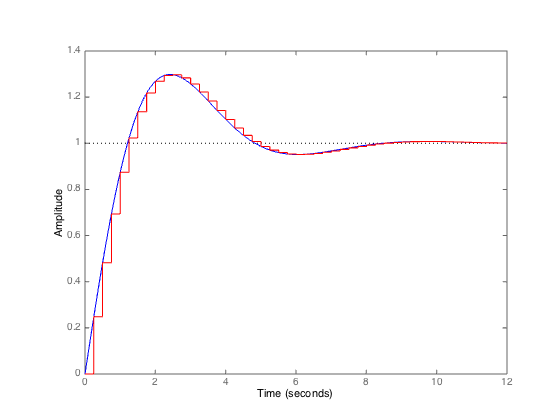
\includegraphics[width=1\linewidth]{vb1}
		\end{figure}
		\end{column}
	\end{columns}
\end{frame}

\begin{frame}
	\frametitle{First-order hold equivalent}
	\begin{example}
		Given:\\
		$H(s) = \frac{s + 1}{s^{2} + s + 1}$\\
		Sampling time = 0.25033sec\\
		\vspace{1em}
		MATLAB commands:
	
		H = tf([1 1],[1 1 1])	\textcolor{gray}{we define the system H by its transfer function} \\
		Hd = c2d(H,$0.25033$,'foh')	\textcolor{gray}{we calculate the discrete-time model}\\
		\vspace{1em}
		Result:
		$H_{foh}(z) = \frac{0.1245z^{2} + 0.02752z - 0.09691}{z^{2} - 1.723z + 0.7785}$
	\end{example}
\end{frame}

\begin{frame}
	\frametitle{First-order hold equivalent (impulse and step response)}
	\vspace{-0.7em}
	\begin{columns}
		\begin{column}{0.5\textwidth}
			\begin{figure}
				\centering
				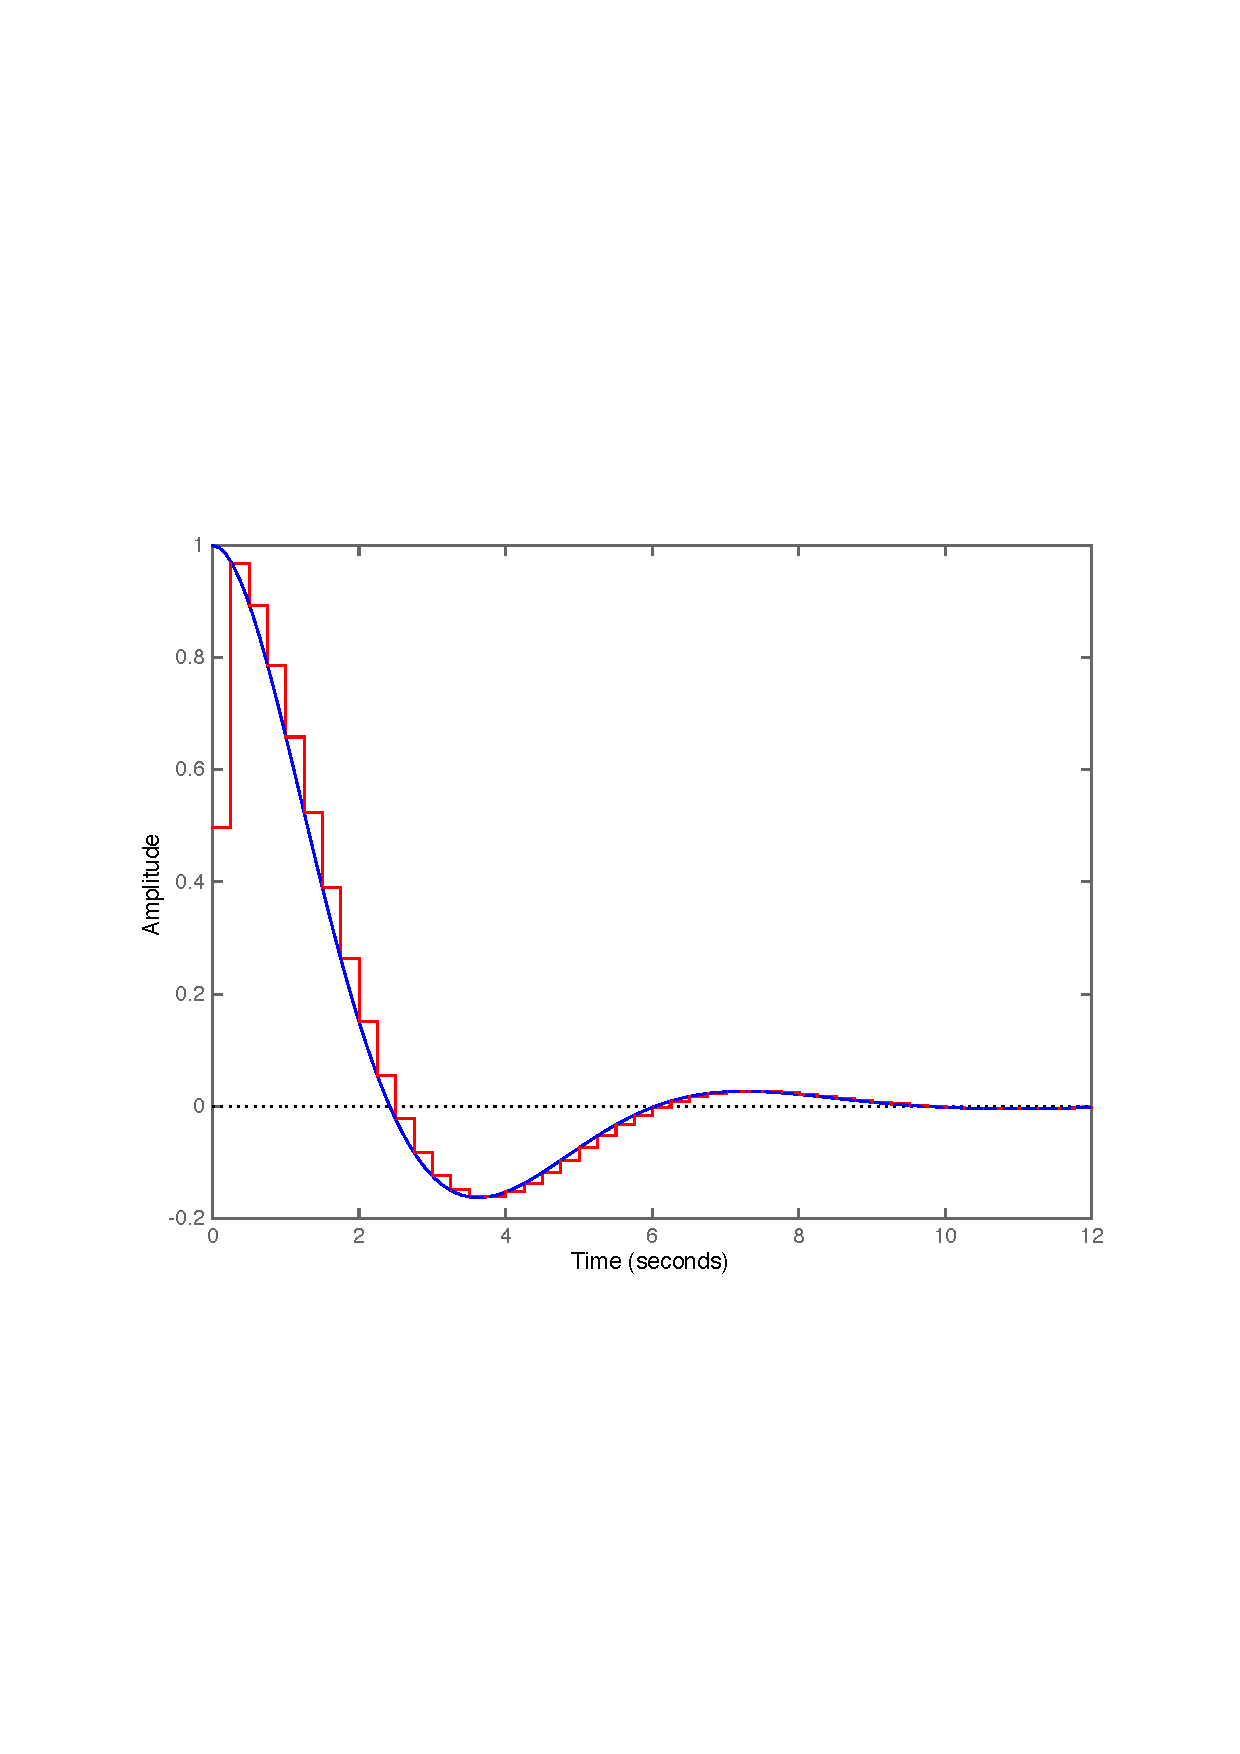
\includegraphics[width=1\linewidth]{vb2I}
			\end{figure}
		\end{column}
		\begin{column}{0.5\textwidth}
			\begin{figure}
				\centering
				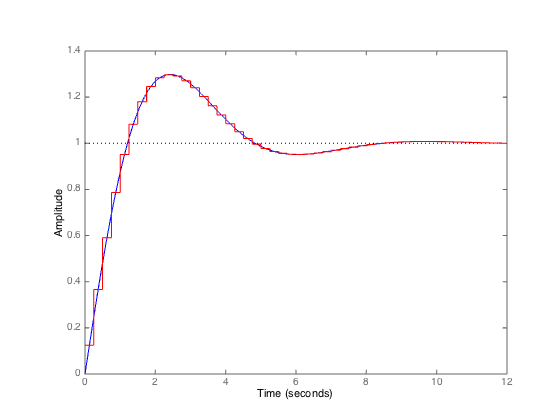
\includegraphics[width=1\linewidth]{vb2}
			\end{figure}
		\end{column}
	\end{columns}
\end{frame}

\begin{frame}
	\frametitle{Impulse invariant rule}
	\begin{example}
		Given:\\
		$H(s) = \frac{s + 1}{s^{2} + s + 1}$\\
		Sampling time = 0.25033sec\\
		\vspace{1em}
		MATLAB commands:
		
		H = tf([1 1],[1 1 1]) \textcolor{gray}{we define the system H by its transfer function} \\
		Hd = c2d(H,$0.25033$,'impuls')	\textcolor{gray}{we calculate the discrete-time model}\\
		\vspace{1em}
		Result:
		$H_{impulse}(z) = \frac{0.2503z^{2} - 0.1883z}{z^{2} - 1.723z + 0.7785}$
	\end{example}
\end{frame}

\begin{frame}
	\frametitle{Impuls invariant rule (impulse and step response)}
	\vspace{-0.7em}
	\begin{columns}
		\begin{column}{0.5\textwidth}
			\begin{figure}
				\centering
				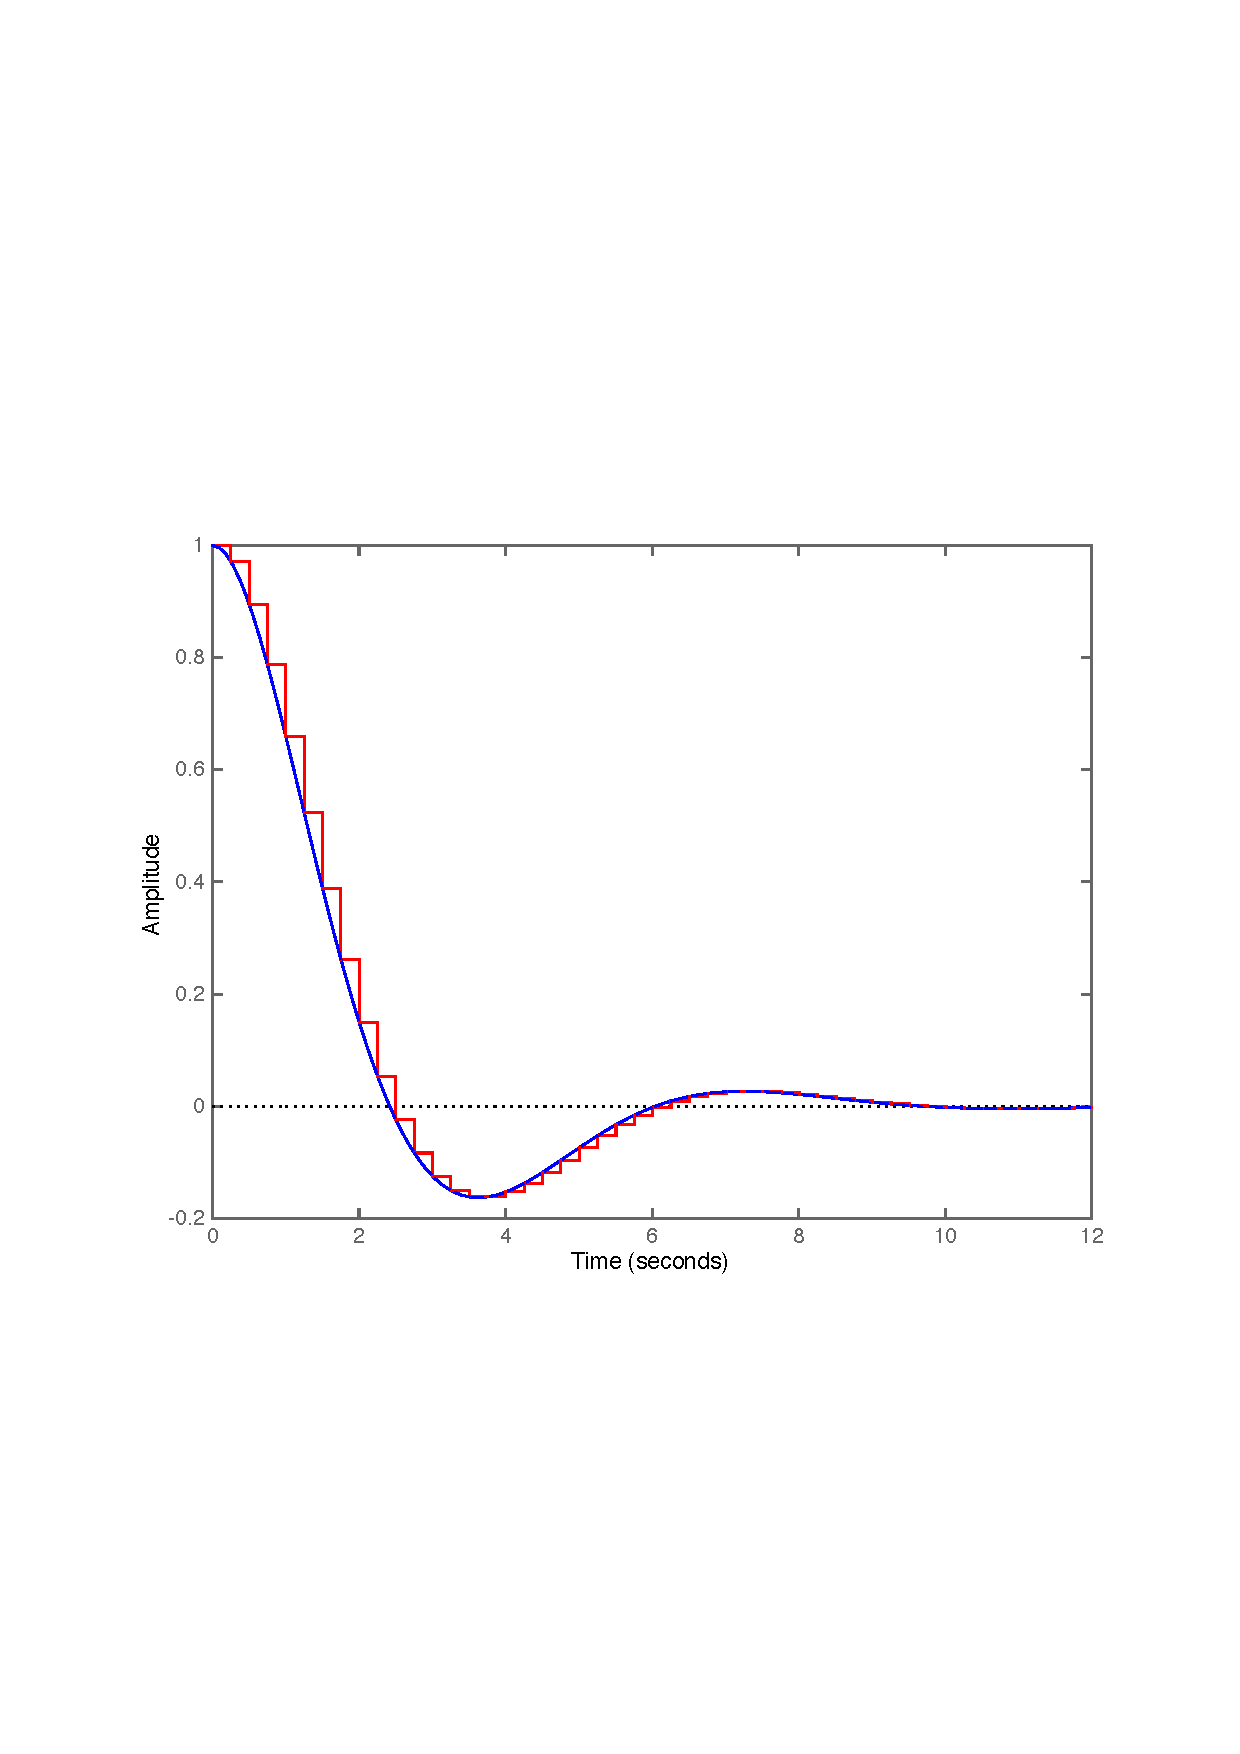
\includegraphics[width=1\linewidth]{vb3I}
			\end{figure}
		\end{column}
		\begin{column}{0.5\textwidth}
			\begin{figure}
				\centering
				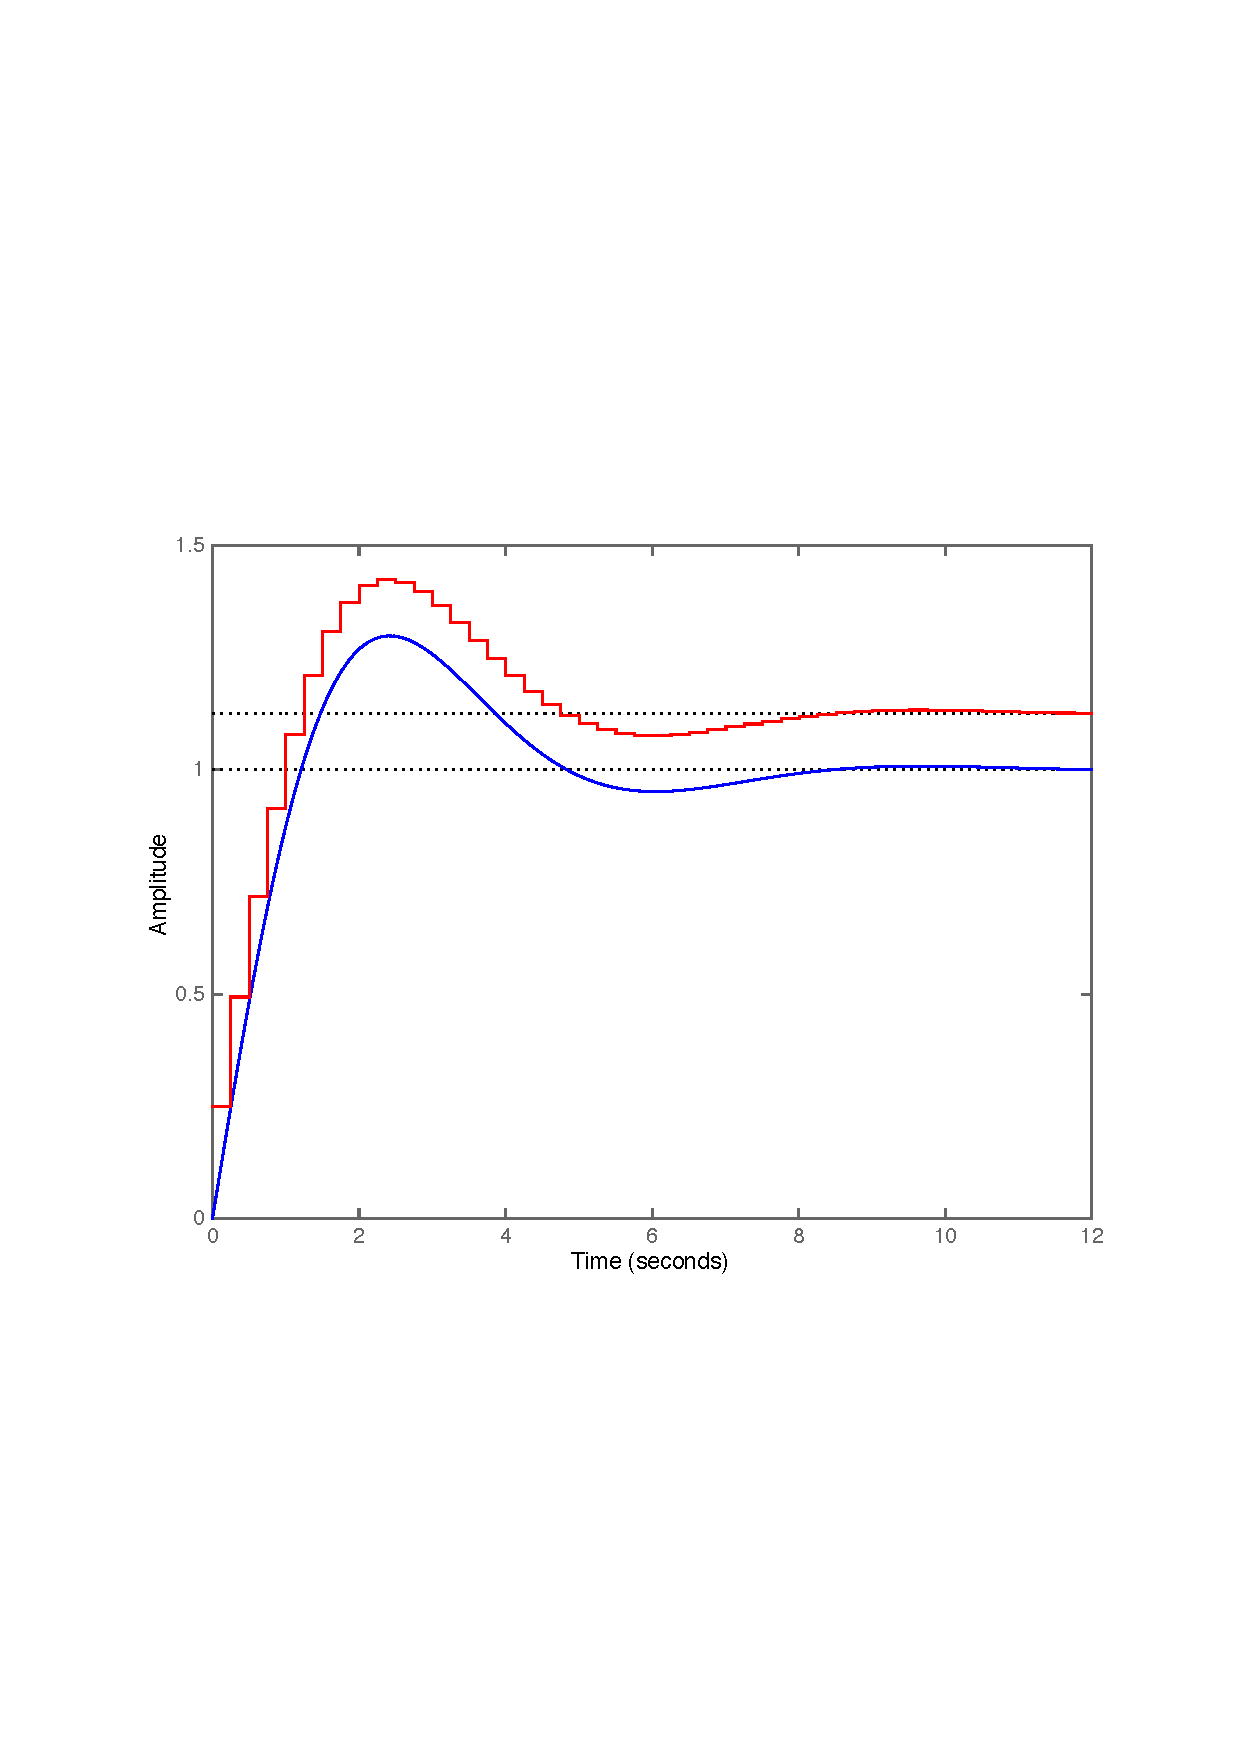
\includegraphics[width=1\linewidth]{vb3}
			\end{figure}
		\end{column}
	\end{columns}
\end{frame}

\begin{frame}
	\frametitle{Zero-pole equivalent}
	\begin{example}
		Given:\\
		$H(s) = \frac{s + 1}{s^{2} + s + 1}$\\
		Sampling time = 0.25033sec\\
		\vspace{1em}
		MATLAB commands:
		
		H = tf([1 1],[1 1 1]) \textcolor{gray}{we define the system H by its transfer function} \\
		Hd = c2d(H,$0.25033$,'matched')	\textcolor{gray}{we calculate the discrete-time model}\\
		\vspace{1em}
		Result: 
		$H_{matched}(z) = \frac{0.249z - 0.1939}{z^{2} - 1.723z + 0.7785}$
	\end{example}
\end{frame}

\begin{frame}
	\frametitle{Zero-pole equivalent (impulse and step response)}
	\vspace{-0.7em}
	\begin{columns}
		\begin{column}{0.5\textwidth}
			\begin{figure}
				\centering
				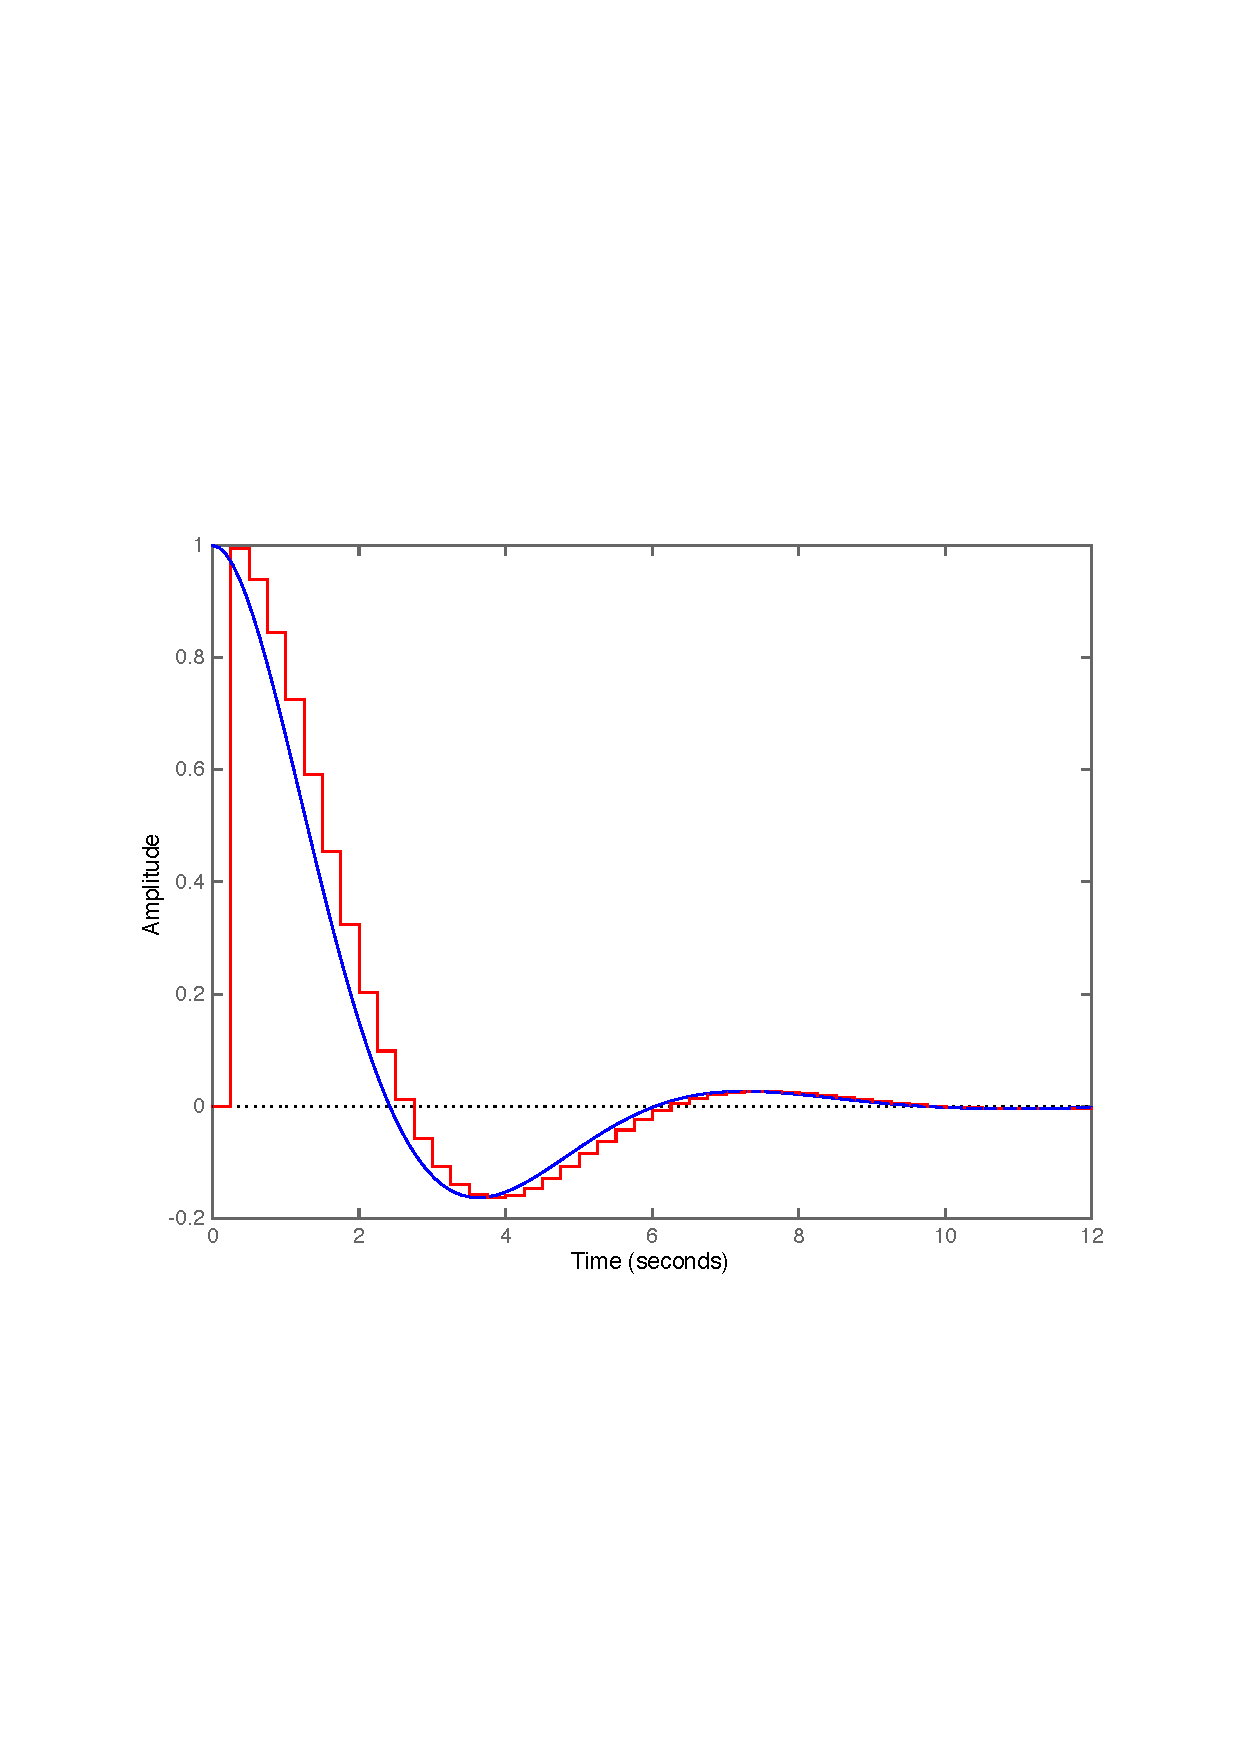
\includegraphics[width=1\linewidth]{vb4I}
			\end{figure}
		\end{column}
		\begin{column}{0.5\textwidth}
			\begin{figure}
				\centering
				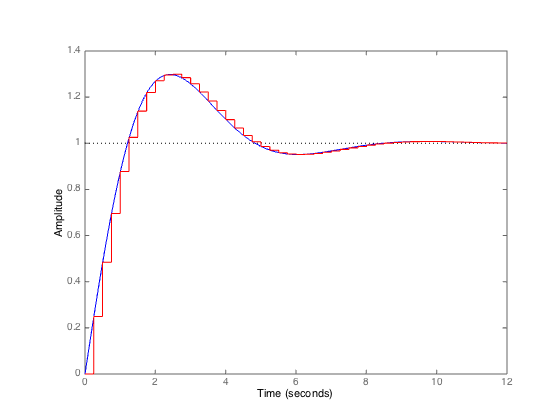
\includegraphics[width=1\linewidth]{vb4}
			\end{figure}
		\end{column}
	\end{columns}
\end{frame}

\begin{frame}
	\frametitle{Exercise 2 with MATLAB}
	\begin{block}{Exercise 2}
		We will now apply the bilinear rule with and without prewarping on the same continuous system: $H(s) = \frac{s^{2} + 0.5s + 9}{s^{2} + 5s + 1}$\\
		\vspace{0.5em}
		Criteria: 
		\begin{enumerate}
			\item The sampling time is chosen to be 0.5 seconds;\\
			\item The discrete system must have the same behaviour as the continuous one at 3rad/s.
		\end{enumerate}
		\vspace{0.5em}
		The last criteria applies to this specific exercise. It is possible that the parity of the magnitude, of the discrete and the continuous system, at a different frequency (e.g. the peak frequency) is required.
	\end{block}	
\end{frame}
		
\begin{frame}
	\frametitle{Tustin rule}
	\begin{example}
		Given:\\
		$H(s) = \frac{s^{2} + 0.5s + 9}{s^{2} + 5s + 1}$\\
		Sampling time = 0.5sec\\
		\vspace{1em}
		MATLAB commands:\\
		
		H = tf([1,0.5,9],[1,5,9])	\textcolor{gray}{definition of the system H} \\
		Hdt = c2d(H,0.5,'tustin')	\textcolor{gray}{we calculate the discrete-time model}\\
		\vspace{1em}
		Result: 
		$H_{Tustin}(z) = \frac{0.6z^{2} - 0.3111z + 0.5111}{z^{2} -  0.3111z + 0.1111}$
	\end{example}
\end{frame}

\begin{frame}
	\frametitle{Tustin rule (bode plot)}
	\vspace{-0.7em}
	\begin{figure}
		\centering
		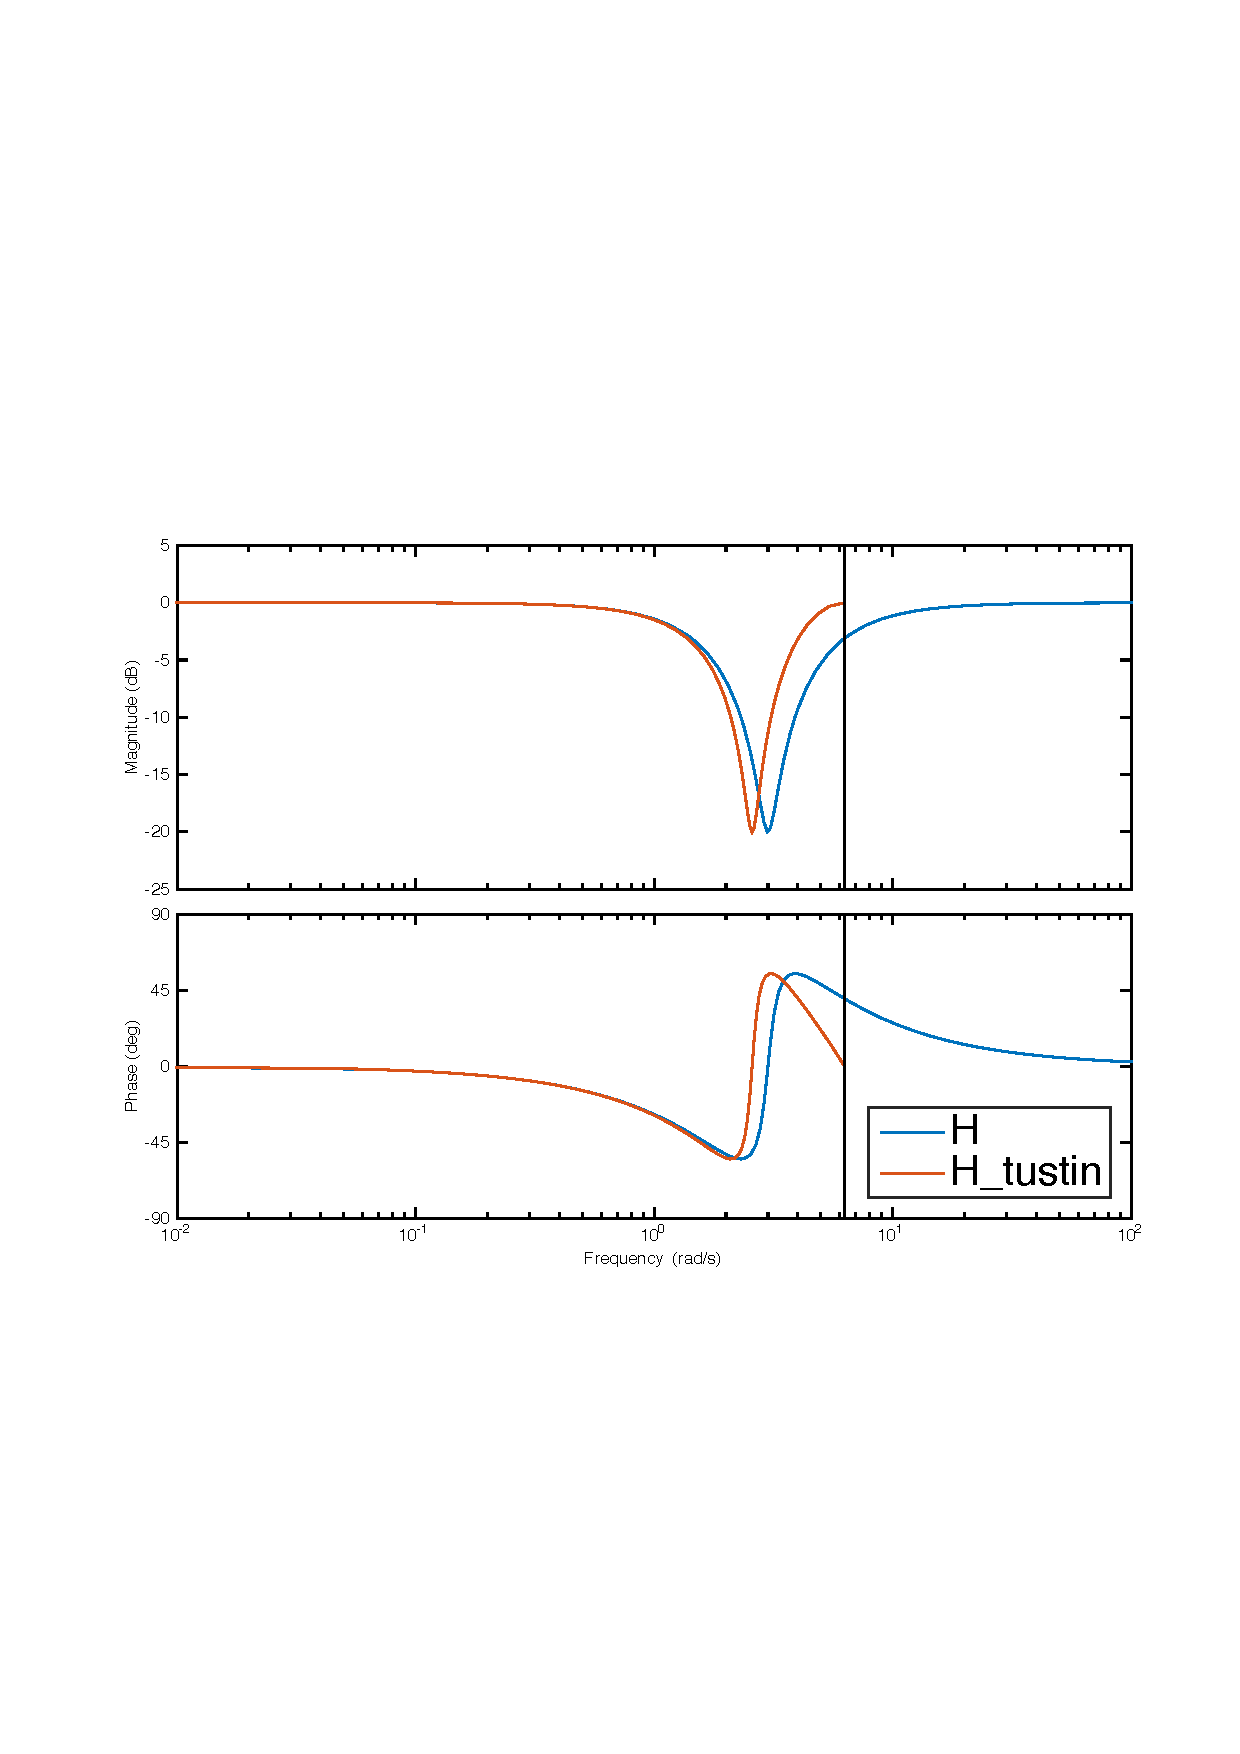
\includegraphics[width=0.9\linewidth]{distortion_bode2}
	\end{figure}
\end{frame}

\begin{frame}
	\frametitle{Tustin rule with prewarping}
	\begin{example}
		Given:\\
		$H(s) = \frac{s^{2} + 0.5s + 9}{s^{2} + 5s + 1}$\\
		Sampling time = 0.5sec\\
		\vspace{1em}
		MATLAB commands:\\
		H = tf([1,0.5,9],[1,5,9])	\textcolor{gray}{definition of the system H} \\
		damp(H)	\textcolor{gray}{results in 3.0Hz} \\
		discopts = c2dOptions('Method','tustin','PrewarpFrequency',3.0)	\textcolor{gray}{at the prewarpfrequency, the discrete-time model will have the same behavior as the continuous-time one}\\
		Hdtp = c2d(H,0.5,discopts)	\textcolor{gray}{we calculate the discrete-time model}\\
		\vspace{1em}
		Result:
		$H_{TustinPrewarp}(z) = \frac{0.5915z^{2} - 0.07726z + 0.5007}{z^{2} - 0.07726z + 0.09215}$
	\end{example}
\end{frame}

\begin{frame}
	\frametitle{Tustin rule with prewarping (bode plot)}
	\vspace{-0.7em}
	\begin{figure}
		\centering
		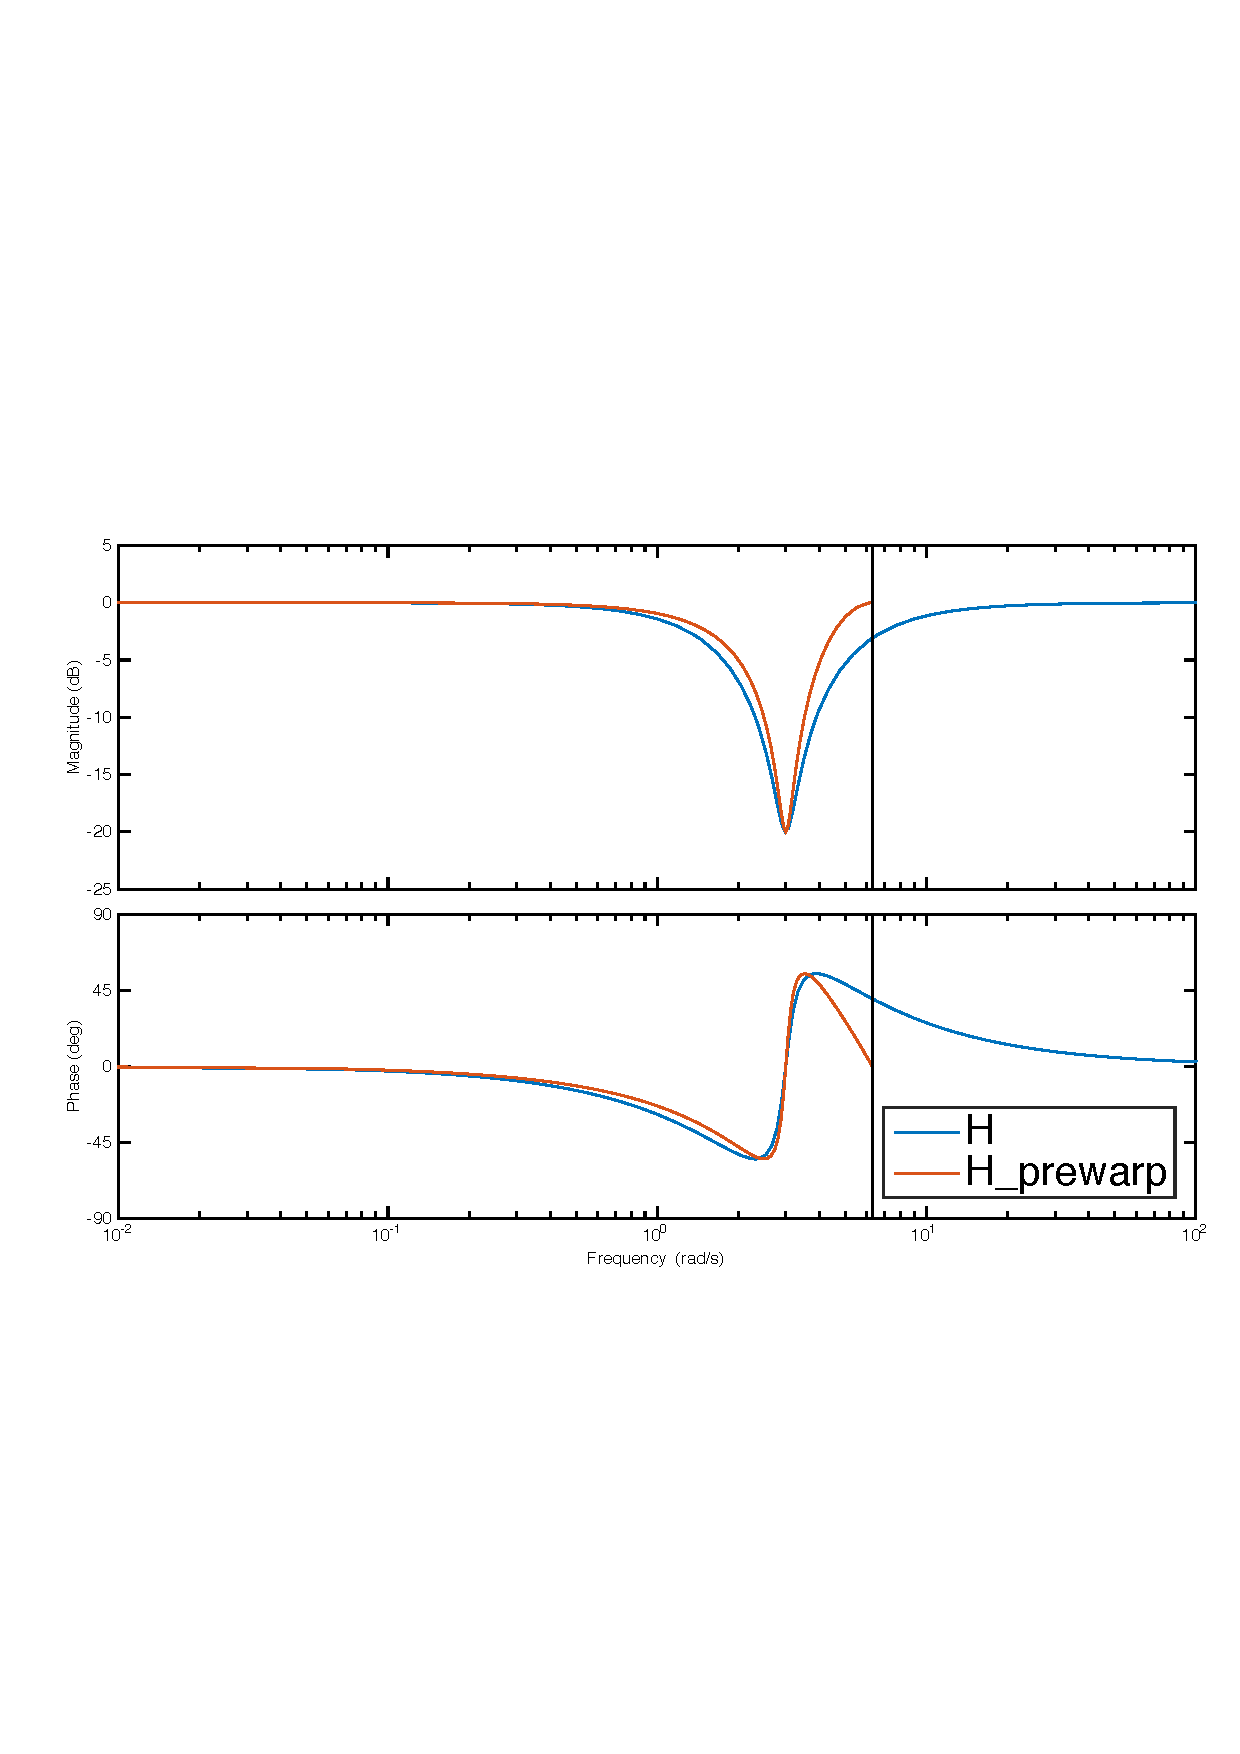
\includegraphics[width=1\linewidth]{distortion_bode3}
	\end{figure}
\end{frame}